\documentclass[slides]{beamer} %switch "slides" to "handout" for printing out
%\documentclass[handout]{beamer}

%packages
%\usepackage{latexsym}
\usepackage{graphicx}
\usepackage{color}
\usepackage{amsmath}
\usepackage{dsfont}
%\usepackage{placeins}
\usepackage{amssymb}
\usepackage{wasysym}
%\usepackage{abstract}
\usepackage{hyperref}
\usepackage{cancel}
%\usepackage[margin=1.05in]{geometry}
%\usepackage{enumerate}
\usepackage{listings}
\usepackage{mathdots}
\usepackage{ulem}
\usepackage{array}
\usepackage{algorithm}
\usepackage{algorithmic}
\usepackage{textcomp}
\usepackage{phaistos}
\usepackage{fancyvrb}
\usepackage{subfigure}
\usepackage[final]{movie15}

\newcommand{\qu}[1]{``#1''}
\newcommand{\centeredimage}[2]{\begin{figure}[htp]\centering\includegraphics[width=#1in]{images/#2}\end{figure}}

\newcommand\verbbf[1]{\colorbox{yellow}{#1}}

\newcommand{\treet}[1]{\text{\scriptsize \PHplaneTree}_{#1}}
\newcommand{\treeleaft}[1]{\text{\scriptsize \PHplaneTree}_{#1}^{\text{\tiny \textleaf}}}
\newcommand{\leaf}{\text{\scriptsize \textleaf}}

\lstset{language = R, numbers = left, backgroundcolor = \color{backgcode}, title = \lstname, breaklines = true, basicstyle = \small, commentstyle = \footnotesize\color{Brown}, stringstyle = \ttfamily, tabsize = 2, fontadjust = true, showspaces = false, showstringspaces = false, texcl = true, numbers = none}

\newcounter{probnum}
\setcounter{probnum}{1}

%create definition to allow local margin changes
\def\changemargin#1#2{\list{}{\rightmargin#2\leftmargin#1}\item[]}
\let\endchangemargin=\endlist 

%allow equations to span multiple pages
\allowdisplaybreaks

%define colors and color typesetting conveniences
\definecolor{gray}{rgb}{0.5,0.5,0.5}
\newcommand{\ingray}[1]{\color{gray}#1 \color{black}}
\definecolor{black}{rgb}{0,0,0}
\definecolor{white}{rgb}{1,1,1}
\definecolor{blue}{rgb}{0,0,0.7}
\newcommand{\inblue}[1]{\color{blue}#1 \color{black}}
\definecolor{green}{rgb}{0.133,0.545,0.133}
\newcommand{\ingreen}[1]{\color{green}#1 \color{black}}
\definecolor{yellow}{rgb}{1,0.549,0}
\newcommand{\inyellow}[1]{\color{yellow}#1 \color{black}}
\definecolor{red}{rgb}{1,0.133,0.133}
\newcommand{\inred}[1]{\color{red}#1 \color{black}}
\definecolor{purple}{rgb}{0.58,0,0.827}
\newcommand{\inpurple}[1]{\color{purple}#1 \color{black}}
\definecolor{backgcode}{rgb}{0.97,0.97,0.8}
\definecolor{Brown}{cmyk}{0,0.81,1,0.60}
\definecolor{OliveGreen}{cmyk}{0.64,0,0.95,0.40}
\definecolor{CadetBlue}{cmyk}{0.62,0.57,0.23,0}

%define new math operators
\DeclareMathOperator*{\argmax}{arg\,max~}
\DeclareMathOperator*{\argmin}{arg\,min~}
\DeclareMathOperator*{\argsup}{arg\,sup~}
\DeclareMathOperator*{\arginf}{arg\,inf~}
\DeclareMathOperator*{\convolution}{\text{\Huge{$\ast$}}}
\newcommand{\infconv}[2]{\convolution^\infty_{#1 = 1} #2}
%true functions

%%%% GENERAL SHORTCUTS

%shortcuts for pure typesetting conveniences
\newcommand{\bv}[1]{\boldsymbol{#1}}

%shortcuts for compound constants
\newcommand{\BetaDistrConst}{\dfrac{\Gamma(\alpha + \beta)}{\Gamma(\alpha)\Gamma(\beta)}}
\newcommand{\NormDistrConst}{\dfrac{1}{\sqrt{2\pi\sigma^2}}}

%shortcuts for conventional symbols
\newcommand{\tsq}{\tau^2}
\newcommand{\tsqh}{\hat{\tau}^2}
\newcommand{\sigsq}{\sigma^2}
\newcommand{\sigsqsq}{\parens{\sigma^2}^2}
\newcommand{\sigsqovern}{\dfrac{\sigsq}{n}}
\newcommand{\tausq}{\tau^2}
\newcommand{\tausqalpha}{\tau^2_\alpha}
\newcommand{\tausqbeta}{\tau^2_\beta}
\newcommand{\tausqsigma}{\tau^2_\sigma}
\newcommand{\betasq}{\beta^2}
\newcommand{\sigsqvec}{\bv{\sigma}^2}
\newcommand{\sigsqhat}{\hat{\sigma}^2}
\newcommand{\Omegahat}{\hat{\Omega}}
\newcommand{\sigsqhatmlebayes}{\sigsqhat_{\text{Bayes, MLE}}}
\newcommand{\sigsqhatmle}[1]{\sigsqhat_{#1, \text{MLE}}}
\newcommand{\bSigma}{\bv{\Sigma}}
\newcommand{\bSigmainv}{\bSigma^{-1}}
\newcommand{\gammavec}{\bv{\gamma}}
\newcommand{\thetavec}{\bv{\theta}}
\newcommand{\thetahat}{\hat{\theta}}
\newcommand{\thetavechat}{\hat{\thetavec}}
\newcommand{\thetahatmle}{\hat{\theta}_{\mathrm{MLE}}}
\newcommand{\thetavechatmle}{\hat{\thetavec}_{\mathrm{MLE}}}
\newcommand{\pihatmle}{\hat{\pi}_{\mathrm{MLE}}}
\newcommand{\muhat}{\hat{\mu}}
\newcommand{\musq}{\mu^2}
\newcommand{\muvec}{\bv{\mu}}
\newcommand{\pivec}{\bv{\pi}}
\newcommand{\muhatmle}{\muhat_{\text{MLE}}}
\newcommand{\lambdahat}{\hat{\lambda}}
\newcommand{\lambdahatmle}{\lambdahat_{\text{MLE}}}
\newcommand{\lambdahatmleone}{\lambdahat_{\text{MLE}, 1}}
\newcommand{\lambdahatmletwo}{\lambdahat_{\text{MLE}, 2}}
\newcommand{\etavec}{\bv{\eta}}
\newcommand{\alphavec}{\bv{\alpha}}
\newcommand{\minimaxdec}{\delta^*_{\mathrm{mm}}}
\newcommand{\ybar}{\bar{y}}
\newcommand{\Ybar}{\bar{Y}}
\newcommand{\xbar}{\bar{x}}
\newcommand{\Xbar}{\bar{X}}
\newcommand{\zbar}{\bar{z}}
\newcommand{\Zbar}{\bar{Z}}

\newcommand{\iid}{~{\buildrel iid \over \sim}~}
\newcommand{\inddist}{~{\buildrel ind \over \sim}~}
\newcommand{\approxdist}{~~{\buildrel approx \over \sim}~~}
\newcommand{\equalsindist}{~{\buildrel d \over =}~}
\newcommand{\equalsquestion}{~{\buildrel ? \over =}~}
\newcommand{\geqquestion}{~{\buildrel ? \over \geq}~}
\newcommand{\lik}[1]{L\parens{#1}}
\newcommand{\loglik}[1]{\ell\parens{#1}}
\newcommand{\thetahatkminone}{\thetahat^{(k-1)}}
\newcommand{\thetahatkplusone}{\thetahat^{(k+1)}}
\newcommand{\thetahatk}{\thetahat^{(k)}}
\newcommand{\half}{\frac{1}{2}}
\newcommand{\third}{\frac{1}{3}}
\newcommand{\twothirds}{\frac{2}{3}}
\newcommand{\fourth}{\frac{1}{4}}
\newcommand{\fifth}{\frac{1}{5}}
\newcommand{\sixth}{\frac{1}{6}}

%shortcuts for vector and matrix notation
\newcommand{\A}{\bv{A}}
\newcommand{\At}{\A^T}
\newcommand{\Ainv}{\inverse{\A}}
\newcommand{\B}{\bv{B}}
\newcommand{\C}{\bv{C}}
\newcommand{\D}{\bv{D}}
\newcommand{\K}{\bv{K}}
\newcommand{\Kt}{\K^T}
\newcommand{\Kinv}{\inverse{K}}
\newcommand{\Kinvt}{(\Kinv)^T}
\newcommand{\M}{\bv{M}}
\newcommand{\Bt}{\B^T}
\newcommand{\Q}{\bv{Q}}
\newcommand{\E}{\bv{E}}
\newcommand{\Et}{\E^\top}
\newcommand{\Qt}{\Q^T}
\newcommand{\R}{\bv{R}}
\newcommand{\Rt}{\R^\top}
\newcommand{\Z}{\bv{Z}}
\newcommand{\X}{\bv{X}}
\renewcommand{\H}{\bv{H}}
\newcommand{\Xsub}{\X_{\text{(sub)}}}
\newcommand{\Xsubadj}{\X_{\text{(sub,adj)}}}
\newcommand{\I}{\bv{I}}
\newcommand{\J}{\bv{J}}
\newcommand{\0}{\bv{0}}
\newcommand{\1}{\bv{1}}
\newcommand{\Y}{\bv{Y}}
\newcommand{\Yt}{\Y^\top}
\newcommand{\tvec}{\bv{t}}
\newcommand{\sigsqI}{\sigsq\I}
\renewcommand{\P}{\bv{P}}
\newcommand{\Psub}{\P_{\text{(sub)}}}
\newcommand{\Pt}{\P^T}
\newcommand{\Pii}{P_{ii}}
\newcommand{\Pij}{P_{ij}}
\newcommand{\IminP}{(\I-\P)}
\newcommand{\Xt}{\bv{X}^T}
\newcommand{\XtX}{\Xt\X}
\newcommand{\XtXinv}{\parens{\Xt\X}^{-1}}
\newcommand{\XtXinvXt}{\XtXinv\Xt}
\newcommand{\XXtXinvXt}{\X\XtXinvXt}
\newcommand{\x}{\bv{x}}
\newcommand{\onevec}{\bv{1}}
\newcommand{\zerovec}{\bv{0}}
\newcommand{\onevectr}{\onevec^\top}
\newcommand{\oneton}{1, \ldots, n}
\newcommand{\yoneton}{y_1, \ldots, y_n}
\newcommand{\yonetonorder}{y_{(1)}, \ldots, y_{(n)}}
\newcommand{\Yoneton}{Y_1, \ldots, Y_n}
\newcommand{\iinoneton}{i \in \braces{\oneton}}
\newcommand{\onetom}{1, \ldots, m}
\newcommand{\jinonetom}{j \in \braces{\onetom}}
\newcommand{\xoneton}{x_1, \ldots, x_n}
\newcommand{\Xoneton}{X_1, \ldots, X_n}
\newcommand{\xt}{\x^T}
\newcommand{\y}{\bv{y}}
\newcommand{\yt}{\y^T}
\newcommand{\n}{\bv{n}}
\renewcommand{\c}{\bv{c}}
\newcommand{\ct}{\c^T}
\newcommand{\tstar}{\bv{t}^*}
\renewcommand{\u}{\bv{u}}
\renewcommand{\v}{\bv{v}}
\renewcommand{\a}{\bv{a}}
\newcommand{\s}{\bv{s}}
\newcommand{\yadj}{\y_{\text{(adj)}}}
\newcommand{\xjadj}{\x_{j\text{(adj)}}}
\newcommand{\xjadjM}{\x_{j \perp M}}
\newcommand{\yhat}{\hat{\y}}
\newcommand{\yhatsub}{\yhat_{\text{(sub)}}}
\newcommand{\yhatstar}{\yhat^*}
\newcommand{\yhatstarnew}{\yhatstar_{\text{new}}}
\newcommand{\z}{\bv{z}}
\newcommand{\zt}{\z^T}
\newcommand{\bb}{\bv{b}}
\newcommand{\bbt}{\bb^T}
\newcommand{\bbeta}{\bv{\beta}}
\newcommand{\beps}{\bv{\epsilon}}
\newcommand{\bepst}{\beps^T}
\newcommand{\e}{\bv{e}}
\newcommand{\Mofy}{\M(\y)}
\newcommand{\KofAlpha}{K(\alpha)}
\newcommand{\ellset}{\mathcal{L}}
\newcommand{\oneminalph}{1-\alpha}
\newcommand{\SSE}{\text{SSE}}
\newcommand{\SSEsub}{\text{SSE}_{\text{(sub)}}}
\newcommand{\MSE}{\text{MSE}}
\newcommand{\RMSE}{\text{RMSE}}
\newcommand{\SSR}{\text{SSR}}
\newcommand{\SST}{\text{SST}}
\newcommand{\JSest}{\delta_{\text{JS}}(\x)}
\newcommand{\Bayesest}{\delta_{\text{Bayes}}(\x)}
\newcommand{\EmpBayesest}{\delta_{\text{EmpBayes}}(\x)}
\newcommand{\BLUPest}{\delta_{\text{BLUP}}}
\newcommand{\MLEest}[1]{\hat{#1}_{\text{MLE}}}

%shortcuts for Linear Algebra stuff (i.e. vectors and matrices)
\newcommand{\twovec}[2]{\bracks{\begin{array}{c} #1 \\ #2 \end{array}}}
\newcommand{\threevec}[3]{\bracks{\begin{array}{c} #1 \\ #2 \\ #3 \end{array}}}
\newcommand{\fivevec}[5]{\bracks{\begin{array}{c} #1 \\ #2 \\ #3 \\ #4 \\ #5 \end{array}}}
\newcommand{\twobytwomat}[4]{\bracks{\begin{array}{cc} #1 & #2 \\ #3 & #4 \end{array}}}
\newcommand{\threebytwomat}[6]{\bracks{\begin{array}{cc} #1 & #2 \\ #3 & #4 \\ #5 & #6 \end{array}}}
\newcommand{\threebythreemat}[9]{\bracks{\begin{array}{ccc} #1 & #2 & #3 \\  #4 & #5 & #6 \\ #7 & #8 & #9 \end{array}}}

%shortcuts for conventional compound symbols
\newcommand{\thetainthetas}{\theta \in \Theta}
\newcommand{\reals}{\mathbb{R}}
\newcommand{\complexes}{\mathbb{C}}
\newcommand{\rationals}{\mathbb{Q}}
\newcommand{\integers}{\mathbb{Z}}
\newcommand{\naturals}{\mathbb{N}}
\newcommand{\forallninN}{~~\forall n \in \naturals}
\newcommand{\forallxinN}[1]{~~\forall #1 \in \reals}
\newcommand{\matrixdims}[2]{\in \reals^{\,#1 \times #2}}
\newcommand{\inRn}[1]{\in \reals^{\,#1}}
\newcommand{\mathimplies}{\quad\Rightarrow\quad}
\newcommand{\mathequiv}{\quad\Leftrightarrow\quad}
\newcommand{\eqncomment}[1]{\quad \text{(#1)}}
\newcommand{\limitn}{\lim_{n \rightarrow \infty}}
\newcommand{\limitN}{\lim_{N \rightarrow \infty}}
\newcommand{\limitd}{\lim_{d \rightarrow \infty}}
\newcommand{\limitt}{\lim_{t \rightarrow \infty}}
\newcommand{\limitsupn}{\limsup_{n \rightarrow \infty}~}
\newcommand{\limitinfn}{\liminf_{n \rightarrow \infty}~}
\newcommand{\limitk}{\lim_{k \rightarrow \infty}}
\newcommand{\limsupn}{\limsup_{n \rightarrow \infty}}
\newcommand{\limsupk}{\limsup_{k \rightarrow \infty}}
\newcommand{\floor}[1]{\left\lfloor #1 \right\rfloor}
\newcommand{\ceil}[1]{\left\lceil #1 \right\rceil}

%shortcuts for environments
\newcommand{\beqn}{\vspace{-0.25cm}\begin{eqnarray*}}
\newcommand{\eeqn}{\end{eqnarray*}}
\newcommand{\bneqn}{\vspace{-0.25cm}\begin{eqnarray}}
\newcommand{\eneqn}{\end{eqnarray}}

\newcommand{\beans}{\color{blue} \beqn  \text{Ans:}~~~}
\newcommand{\eeans}{\eeqn \color{black}}

%shortcuts for mini environments
\newcommand{\parens}[1]{\left(#1\right)}
\newcommand{\squared}[1]{\parens{#1}^2}
\newcommand{\angbraces}[1]{\left<#1\right>}
\newcommand{\tothepow}[2]{\parens{#1}^{#2}}
\newcommand{\prob}[1]{\mathbb{P}\parens{#1}}
\newcommand{\probsub}[2]{\mathbb{P}_{\text{#1}}\parens{#2}}
\newcommand{\cprob}[2]{\prob{#1~|~#2}}
\newcommand{\littleo}[1]{o\parens{#1}}
\newcommand{\bigo}[1]{O\parens{#1}}
\newcommand{\Lp}[1]{\mathbb{L}^{#1}}
\renewcommand{\arcsin}[1]{\text{arcsin}\parens{#1}}
\newcommand{\prodonen}[2]{\prod_{#1=1}^n #2}
\newcommand{\mysum}[4]{\sum_{#1=#2}^{#3} #4}
\newcommand{\sumonen}[2]{\sum_{#1=1}^n #2}
\newcommand{\infsum}[2]{\sum_{#1=1}^\infty #2}
\newcommand{\infprod}[2]{\prod_{#1=1}^\infty #2}
\newcommand{\infunion}[2]{\bigcup_{#1=1}^\infty #2}
\newcommand{\infinter}[2]{\bigcap_{#1=1}^\infty #2}
\newcommand{\infintegral}[2]{\int^\infty_{-\infty} #2 ~\text{d}#1}
\newcommand{\supthetas}[1]{\sup_{\thetainthetas}\braces{#1}}
\newcommand{\bracks}[1]{\left[#1\right]}
\newcommand{\braces}[1]{\left\{#1\right\}}
\newcommand{\set}[1]{\left\{#1\right\}}
\newcommand{\abss}[1]{\left|#1\right|}
\newcommand{\norm}[1]{\left|\left|#1\right|\right|}
\newcommand{\normsq}[1]{\norm{#1}^2}
\newcommand{\inverse}[1]{\parens{#1}^{-1}}
\newcommand{\rowof}[2]{\parens{#1}_{#2\cdot}}

%shortcuts for functionals
\newcommand{\realcomp}[1]{\text{Re}\bracks{#1}}
\newcommand{\imagcomp}[1]{\text{Im}\bracks{#1}}
\newcommand{\range}[1]{\text{range}\bracks{#1}}
\newcommand{\colsp}[1]{\text{colsp}\bracks{#1}}
\newcommand{\rowsp}[1]{\text{rowsp}\bracks{#1}}
\newcommand{\tr}[1]{\text{tr}\bracks{#1}}
\newcommand{\diag}[1]{\text{diag}\bracks{#1}}
\newcommand{\rank}[1]{\text{rank}\bracks{#1}}
\newcommand{\proj}[2]{\text{Proj}_{#1}\bracks{#2}}
\newcommand{\projcolspX}[1]{\text{Proj}_{\colsp{\X}}\bracks{#1}}
\newcommand{\median}[1]{\text{median}\bracks{#1}}
\newcommand{\mean}[1]{\text{mean}\bracks{#1}}
\newcommand{\dime}[1]{\text{dim}\bracks{#1}}
\renewcommand{\det}[1]{\text{det}\bracks{#1}}
\newcommand{\expe}[1]{\mathbb{E}\bracks{#1}}
\newcommand{\cexpe}[2]{\expe{#1 ~ | ~ #2}}
\newcommand{\expeabs}[1]{\expe{\abss{#1}}}
\newcommand{\expesub}[2]{\mathbb{E}_{#1}\bracks{#2}}
\newcommand{\indic}[1]{\mathds{1}_{#1}}
\newcommand{\var}[1]{\mathbb{V}\text{ar}\bracks{#1}}
\newcommand{\varhat}[1]{\hat{\mathbb{V}\text{ar}}\bracks{#1}}
\newcommand{\cov}[2]{\mathbb{C}\text{ov}\bracks{#1, #2}}
\newcommand{\corr}[2]{\text{Corr}\bracks{#1, #2}}
\newcommand{\se}[1]{\text{SE}\bracks{#1}}
\newcommand{\seest}[1]{\hat{\text{SE}}\bracks{#1}}
\newcommand{\bias}[1]{\text{Bias}\bracks{#1}}
\newcommand{\partialop}[2]{\dfrac{\partial}{\partial #1}\bracks{#2}}
\newcommand{\secpartialop}[2]{\dfrac{\partial^2}{\partial #1^2}\bracks{#2}}
\newcommand{\mixpartialop}[3]{\dfrac{\partial^2}{\partial #1 \partial #2}\bracks{#3}}

%shortcuts for functions
\renewcommand{\exp}[1]{\mathrm{exp}\parens{#1}}
\renewcommand{\cos}[1]{\text{cos}\parens{#1}}
\renewcommand{\sin}[1]{\text{sin}\parens{#1}}
\newcommand{\sign}[1]{\text{sign}\parens{#1}}
\newcommand{\are}[1]{\mathrm{ARE}\parens{#1}}
\newcommand{\natlog}[1]{\ln\parens{#1}}
\newcommand{\oneover}[1]{\frac{1}{#1}}
\newcommand{\overtwo}[1]{\frac{#1}{2}}
\newcommand{\overn}[1]{\frac{#1}{n}}
\newcommand{\oneoversqrt}[1]{\oneover{\sqrt{#1}}}
\newcommand{\sqd}[1]{\parens{#1}^2}
\newcommand{\loss}[1]{\ell\parens{\theta, #1}}
\newcommand{\losstwo}[2]{\ell\parens{#1, #2}}
\newcommand{\cf}{\phi(t)}

%English language specific shortcuts
\newcommand{\ie}{\textit{i.e.} }
\newcommand{\AKA}{\textit{AKA} }
\renewcommand{\iff}{\textit{iff}}
\newcommand{\eg}{\textit{e.g.} }
\newcommand{\st}{\textit{s.t.} }
\newcommand{\wrt}{\textit{w.r.t.} }
\newcommand{\mathst}{~~\text{\st}~~}
\newcommand{\mathand}{~~\text{and}~~}
\newcommand{\mathor}{~~\text{or}~~}
\newcommand{\ala}{\textit{a la} }
\newcommand{\ppp}{posterior predictive p-value}
\newcommand{\dd}{dataset-to-dataset}

%shortcuts for distribution titles
\newcommand{\logistic}[2]{\mathrm{Logistic}\parens{#1,\,#2}}
\newcommand{\bernoulli}[1]{\mathrm{Bernoulli}\parens{#1}}
\newcommand{\betanot}[2]{\mathrm{Beta}\parens{#1,\,#2}}
\newcommand{\stdbetanot}{\betanot{\alpha}{\beta}}
\newcommand{\multnormnot}[3]{\mathcal{N}_{#1}\parens{#2,\,#3}}
\newcommand{\normnot}[2]{\mathcal{N}\parens{#1,\,#2}}
\newcommand{\classicnormnot}{\normnot{\mu}{\sigsq}}
\newcommand{\stdnormnot}{\normnot{0}{1}}
\newcommand{\uniform}[2]{\mathrm{U}\parens{#1,\,#2}}
\newcommand{\stduniform}{\uniform{0}{1}}
\newcommand{\exponential}[1]{\mathrm{Exp}\parens{#1}}
\newcommand{\stdexponential}{\mathrm{Exp}\parens{1}}
\newcommand{\gammadist}[2]{\mathrm{Gamma}\parens{#1, #2}}
\newcommand{\poisson}[1]{\mathrm{Poisson}\parens{#1}}
\newcommand{\geometric}[1]{\mathrm{Geometric}\parens{#1}}
\newcommand{\binomial}[2]{\mathrm{Binomial}\parens{#1,\,#2}}
\newcommand{\rayleigh}[1]{\mathrm{Rayleigh}\parens{#1}}
\newcommand{\multinomial}[2]{\mathrm{Multinomial}\parens{#1,\,#2}}
\newcommand{\gammanot}[2]{\mathrm{Gamma}\parens{#1,\,#2}}
\newcommand{\cauchynot}[2]{\text{Cauchy}\parens{#1,\,#2}}
\newcommand{\invchisqnot}[1]{\text{Inv}\chisq{#1}}
\newcommand{\invscaledchisqnot}[2]{\text{ScaledInv}\ncchisq{#1}{#2}}
\newcommand{\invgammanot}[2]{\text{InvGamma}\parens{#1,\,#2}}
\newcommand{\chisq}[1]{\chi^2_{#1}}
\newcommand{\ncchisq}[2]{\chi^2_{#1}\parens{#2}}
\newcommand{\ncF}[3]{F_{#1,#2}\parens{#3}}

%shortcuts for PDF's of common distributions
\newcommand{\logisticpdf}[3]{\oneover{#3}\dfrac{\exp{-\dfrac{#1 - #2}{#3}}}{\parens{1+\exp{-\dfrac{#1 - #2}{#3}}}^2}}
\newcommand{\betapdf}[3]{\dfrac{\Gamma(#2 + #3)}{\Gamma(#2)\Gamma(#3)}#1^{#2-1} (1-#1)^{#3-1}}
\newcommand{\normpdf}[3]{\frac{1}{\sqrt{2\pi#3}}\exp{-\frac{1}{2#3}(#1 - #2)^2}}
\newcommand{\normpdfvarone}[2]{\dfrac{1}{\sqrt{2\pi}}e^{-\half(#1 - #2)^2}}
\newcommand{\chisqpdf}[2]{\dfrac{1}{2^{#2/2}\Gamma(#2/2)}\; {#1}^{#2/2-1} e^{-#1/2}}
\newcommand{\invchisqpdf}[2]{\dfrac{2^{-\overtwo{#1}}}{\Gamma(#2/2)}\,{#1}^{-\overtwo{#2}-1}  e^{-\oneover{2 #1}}}
\newcommand{\exponentialpdf}[2]{#2\exp{-#2#1}}
\newcommand{\poissonpdf}[2]{\dfrac{e^{-#1} #1^{#2}}{#2!}}
\newcommand{\binomialpdf}[3]{\binom{#2}{#1}#3^{#1}(1-#3)^{#2-#1}}
\newcommand{\rayleighpdf}[2]{\dfrac{#1}{#2^2}\exp{-\dfrac{#1^2}{2 #2^2}}}
\newcommand{\gammapdf}[3]{\dfrac{#3^#2}{\Gamma\parens{#2}}#1^{#2-1}\exp{-#3 #1}}
\newcommand{\cauchypdf}[3]{\oneover{\pi} \dfrac{#3}{\parens{#1-#2}^2 + #3^2}}
\newcommand{\Gammaf}[1]{\Gamma\parens{#1}}

%shortcuts for miscellaneous typesetting conveniences
\newcommand{\notesref}[1]{\marginpar{\color{gray}\tt #1\color{black}}}

%%%% DOMAIN-SPECIFIC SHORTCUTS

%Real analysis related shortcuts
\newcommand{\zeroonecl}{\bracks{0,1}}
\newcommand{\forallepsgrzero}{\forall \epsilon > 0~~}
\newcommand{\lessthaneps}{< \epsilon}
\newcommand{\fraccomp}[1]{\text{frac}\bracks{#1}}

%Bayesian related shortcuts
\newcommand{\yrep}{y^{\text{rep}}}
\newcommand{\yrepisq}{(\yrep_i)^2}
\newcommand{\yrepvec}{\bv{y}^{\text{rep}}}


%Probability shortcuts
\newcommand{\SigField}{\mathcal{F}}
\newcommand{\ProbMap}{\mathcal{P}}
\newcommand{\probtrinity}{\parens{\Omega, \SigField, \ProbMap}}
\newcommand{\convp}{~{\buildrel p \over \rightarrow}~}
\newcommand{\convLp}[1]{~{\buildrel \Lp{#1} \over \rightarrow}~}
\newcommand{\nconvp}{~{\buildrel p \over \nrightarrow}~}
\newcommand{\convae}{~{\buildrel a.e. \over \longrightarrow}~}
\newcommand{\convau}{~{\buildrel a.u. \over \longrightarrow}~}
\newcommand{\nconvau}{~{\buildrel a.u. \over \nrightarrow}~}
\newcommand{\nconvae}{~{\buildrel a.e. \over \nrightarrow}~}
\newcommand{\convd}{~{\buildrel \mathcal{D} \over \longrightarrow}~}
\newcommand{\nconvd}{~{\buildrel \mathcal{D} \over \nrightarrow}~}
\newcommand{\setequals}{~{\buildrel \text{set} \over =}~}
\newcommand{\withprob}{~~\text{w.p.}~~}
\newcommand{\io}{~~\text{i.o.}}

\newcommand{\Acl}{\bar{A}}
\newcommand{\ENcl}{\bar{E}_N}
\newcommand{\diam}[1]{\text{diam}\parens{#1}}

\newcommand{\taua}{\tau_a}

\newcommand{\myint}[4]{\int_{#2}^{#3} #4 \,\text{d}#1}
\newcommand{\laplacet}[1]{\mathscr{L}\bracks{#1}}
\newcommand{\laplaceinvt}[1]{\mathscr{L}^{-1}\bracks{#1}}
\renewcommand{\min}[1]{\text{min}\braces{#1}}

\newcommand{\Vbar}[1]{\bar{V}\parens{#1}}
\newcommand{\expnegrtau}{\exp{-r\tau}}
\newcommand{\pval}{p_{\text{val}}}
\newcommand{\alphaovertwo}{\overtwo{\alpha}}

%%% problem typesetting
%\newcommand{\problem}{\vspace{0.4cm} \noindent {\large{\textsf{Problem \arabic{probnum}~}}} \addtocounter{probnum}{1}}
%\newcommand{\easyproblem}{\ingreen{\noindent \textsf{Problem \arabic{probnum}~}} \addtocounter{probnum}{1}}
%\newcommand{\intermediateproblem}{\noindent \inyellow{\textsf{Problem \arabic{probnum}~}} \addtocounter{probnum}{1}}
%\newcommand{\hardproblem}{\inred{\noindent \textsf{Problem \arabic{probnum}~}} \addtocounter{probnum}{1}}
%\newcommand{\extracreditproblem}{\noindent \inpurple{\textsf{Problem \arabic{probnum}~}} \addtocounter{probnum}{1}}

\newcommand{\easysubproblem}{\ingreen{\item}}
\newcommand{\intermediatesubproblem}{\inyellow{\item}}
\newcommand{\hardsubproblem}{\inred{\item}}
\newcommand{\extracreditsubproblem}{\inpurple{\item}}
%\renewcommand{\labelenumi}{(\alph{enumi})}

\newcommand{\nonep}{n_{1+}}
\newcommand{\npone}{n_{+1}}
\newcommand{\npp}{n_{++}}
\newcommand{\noneone}{n_{11}}
\newcommand{\nonetwo}{n_{12}}
\newcommand{\ntwoone}{n_{21}}
\newcommand{\ntwotwo}{n_{22}}

\newcommand{\sigmahat}{\hat{\sigma}}
\newcommand{\pihat}{\hat{\pi}}


\newcommand{\probD}{\prob{D}}
\newcommand{\probDC}{\prob{D^C}}
\newcommand{\probE}{\prob{E}}
\newcommand{\probEC}{\prob{E^C}}
\newcommand{\probDE}{\prob{D,E}}
\newcommand{\probDEC}{\prob{D,E^C}}
\newcommand{\probDCE}{\prob{D^C,E}}
\newcommand{\probDCEC}{\prob{D^C,E^C}}

\newcommand{\logit}[1]{\text{logit}\parens{#1}}

\newcommand{\errorrv}{\mathcal{E}}
\newcommand{\berrorrv}{\bv{\errorrv}}
\newcommand{\DIM}{\mathcal{I}}
\newcommand{\trans}[1]{#1^\top}
\newcommand{\transp}[1]{\parens{#1}^\top}



\newcommand{\nr}{n_{R}}
\newcommand{\nrc}{n_{R,C}}
\newcommand{\nrt}{n_{R,T}}
\newcommand{\indicrti}{\indic{R,T,i}}
\newcommand{\indicrtj}{\indic{R,T,j}}
\newcommand{\Dbar}{\bar{D}}
\newcommand{\SsqDbar}{S^2_{\Dbar}}
\newcommand{\SsqR}{S^2_R}
\newcommand{\YbarRT}{\Ybar_{R,T}}
\newcommand{\YbarRC}{\Ybar_{R,C}}
\newcommand{\YbarRTMinusYbarRC}{\YbarRT - \YbarRC}

\newcommand{\dbar}{\bar{d}}
\newcommand{\ssqDbar}{s^2_{\Dbar}}
\newcommand{\ssqR}{s^2_R}
\newcommand{\ybarRT}{\ybar_{R,T}}
\newcommand{\ybarRC}{\ybar_{R,C}}
\newcommand{\ybarRTMinusybarRC}{\ybarRT - \ybarRC}



\newcommand{\sigsqR}{\sigsq_R}
\newcommand{\sigsqDbar}{\sigsq_{\bar{D}}}
\newcommand{\sigsqDeltaYbar}{\sigsq_{\Delta\Ybar}}
\newcommand{\oneovernrtplusoneovernrc}{\oneover{\nrt} + \oneover{\nrc}}
\newcommand{\parensoneovernrtplusoneovernrc}{\parens{\oneovernrtplusoneovernrc}}
\newcommand{\sigsqBT}{\sigsq_{B_T}}
\newcommand{\nrpooled}{n_{R,p}^{-1}} %%change later


\newcommand{\angbrace}[1]{\left<#1\right>}

\usepackage{beamerthemesplit}
%presentation preamble
\usetheme{progressbar}
\usecolortheme{progressbar} 
\usefonttheme{progressbar} 
\useoutertheme{progressbar}
\useinnertheme{progressbar}

\title[The Statistics of Crowdsourcing]{Crowdsourcing for Statisticians\\ Designing Applications and Analyzing Data on MTurk}
\institute[Wharton, Statistics]{*Department of Statistics, The Wharton School, University of Pennsylvania \\
**Department of Computer Science, University of Pennsylvania}
\date{August 5, 2013 \\ \footnotesize{Joint Statistical Meeting Half Day Tutorial}}

\author{Adam Kapelner* and Lyle Ungar**}

%%% GENERAL CROWDSOURCING followed by crowdsourcing for statisticians since in order to do data analysis, you need to understand the data!

\begin{document}


%immediately create a title page
\frame{\titlepage}

\section{Introduction}

%%%%%%%%%%%%%%%%%%%%%%%%%%%%%%%%%%%%%%%%%%%
\begin{frame}\frametitle{Curriculum and Plan}

\scriptsize

\textbf{Overview of Crowdsourcing}
\vspace{-0.1cm}
\begin{itemize}
\item Modern crowdsourcing with emphasis on microlabor for microtasks 
\item Amazon's Mechanical Turk (MTurk) from an employer and worker perspective 
\item What industry professionals and academics use MTurk for \pause
\end{itemize}

\textbf{Survey tasks}
\vspace{-0.1cm}
\begin{itemize}
\item Design and validity of MTurk surveys \pause
\end{itemize}

\textbf{Labeling tasks}
\vspace{-0.1cm}
\begin{itemize}
\item The design and analysis of MTurk \qu{labeling} tasks (with case studies) 
\item Model building and machine learning \pause
\end{itemize}

\textbf{Experimental tasks}
\vspace{-0.1cm}
\begin{itemize}
\item The design of and analysis of MTurk \qu{experimental} tasks (with case studies) 
\item Drawing conclusions from crowdsourced experiments
\end{itemize}

\end{frame}
%%%%%%%%%%%%%%%%%%%%%%%%%%%%%%%%%%%%%%%%%%%

%%%%%%%%%%%%%%%%%%%%%%%%%%%%%%%%%%%%%%%%%%%
\begin{frame}\frametitle{Course Goals}

\begin{block}{What you should be able to do by noon today} \pause
\begin{enumerate}[A]
\item Know what MTurk is used for in academia and industry \textit{and thereby} recognize where crowdsourcing could be useful in your work \pause

\item Use MTurk for survey research \pause

\item For crowdsourced labeling tasks: \pause
\begin{itemize}
\item Evaluate if the labeling task is suitable for crowdsourcing \pause
\item Design the labeling task \pause
\item Analyze the resulting data \pause
\end{itemize}

\item For crowdsourced randomized experiments: \pause
\begin{itemize}
\item Evaluate if the experiment is suitable for crowdsourcing \pause
\item Design the experiment \pause
\item Analyze the resulting data \pause
\end{itemize}
\end{enumerate}
\end{block}

\end{frame}
%%%%%%%%%%%%%%%%%%%%%%%%%%%%%%%%%%%%%%%%%%%

%%%%%%%%%%%%%%%%%%%%%%%%%%%%%%%%%%%%%%%%%%%
\begin{frame}\frametitle{Our crowdsourcing experience. What is yours?}


\begin{center}
\begin{minipage}{0.2\linewidth}
\centering
\centeredimage{0.7}{LyleUngar.jpg}
\end{minipage}
\begin{minipage}{0.78\linewidth}
\scriptsize \textbf{Lyle Ungar} is a professor of Computer and
Information Science at the University of Pennsylvania. His research
group makes extensive use of crowdsourcing for labeling text including tweets, Facebook posts, and word senses 
to support research in natural language processing and psychology.

\end{minipage}
\end{center}

\begin{center}
\begin{minipage}{0.2\linewidth}
\centering
\centeredimage{0.7}{adk1.jpeg}
\end{minipage}
\begin{minipage}{0.78\linewidth}
\scriptsize
\textbf{Adam Kapelner} is a PhD student in Statistics at Wharton focused on crowdsourcing applications. He has published multiple papers using crowdsourced experimentation and labeling data in economics, psychology, and linguistics, including the first paper advocating crowdsourced natural field experiments.
\end{minipage}
\end{center}

\end{frame}
%%%%%%%%%%%%%%%%%%%%%%%%%%%%%%%%%%%%%%%%%%%

%%%%%%%%%%%%%%%%%%%%%%%%%%%%%%%%%%%%%%%%%%%
\begin{frame}\frametitle{What is Crowdsourcing?}

\qu{It’s not outsourcing; it’s crowdsourcing} Howe (2006)

\centeredimage{4}{crowdsourcing.jpg} \pause

\qu{the biggest paradigm shift in innovation since the Industrial Revolution} -Wendy Kaufman, NPR, 2008

\end{frame}
%%%%%%%%%%%%%%%%%%%%%%%%%%%%%%%%%%%%%%%%%%%

%%%%%%%%%%%%%%%%%%%%%%%%%%%%%%%%%%%%%%%%%%%
\begin{frame}\frametitle{Types: I - Wisdom of the Crowd}

 \pause

\begin{itemize}

\item Wikipedia

\centeredimage{1}{wikipedia-logo.jpg} \pause

\item Yahoo Answers

\centeredimage{1}{yahoo_answers.png} \pause

\item Stackoverflow

\centeredimage{1}{stack_overflow_logo.png}

\end{itemize}

\end{frame}
%%%%%%%%%%%%%%%%%%%%%%%%%%%%%%%%%%%%%%%%%%%

%%%%%%%%%%%%%%%%%%%%%%%%%%%%%%%%%%%%%%%%%%%
\begin{frame}\frametitle{Types: II - Crowdfunding}

 \pause

\begin{itemize}

\item Kickstarter / RocketHub / Fundly / IndieGoGo

\centeredimage{3.5}{fundinglogos.jpg} \pause

\item Realty Mogul

\centeredimage{1}{Realty-Mogul.jpg}

\end{itemize}

\end{frame}
%%%%%%%%%%%%%%%%%%%%%%%%%%%%%%%%%%%%%%%%%%%

%%%%%%%%%%%%%%%%%%%%%%%%%%%%%%%%%%%%%%%%%%%
\begin{frame}\frametitle{Types: III - Creative Work}

\pause

\begin{itemize}

\vspace{-0.2cm}
\item 99 Designs, threadless

\vspace{-0.3cm}
\centeredimage{1.2}{99designs_threadless.jpg} \pause
\vspace{-0.1cm}

\item oDesk, eLance, rentacoder, guru

\vspace{-0.1cm}
\centeredimage{1.2}{odesk_elance_rentacoder_guru.jpg} \pause
\vspace{-0.1cm}

\item IdeaBounty and Innocentive

\vspace{-0.2cm}
\centeredimage{1.2}{innocentive_ideabounty.jpg} \pause
\vspace{-0.1cm}

\item Inducement Prize: Ansari-X, DARPA balloon challenge, Netflix Prize, the Nobel?

\vspace{-0.3cm}
\centeredimage{2.5}{nobel_ansari.jpg}

\end{itemize}

\end{frame}
%%%%%%%%%%%%%%%%%%%%%%%%%%%%%%%%%%%%%%%%%%%

%%%%%%%%%%%%%%%%%%%%%%%%%%%%%%%%%%%%%%%%%%%
\begin{frame}\frametitle{Type IV - Microwork / Microlabor}

\pause

\begin{itemize}

\item Amazon's Mechanical Turk (MTurk)

\centeredimage{2}{mturk.png} \pause

\item Specialized: LiveOps, Clickworker, Ahn's ESP Game

\centeredimage{3.5}{liveops_clickworker.jpg} \pause

\item Intermediaries: Crowdflower, Crowdsource, Alegion, Smartsheet

\centeredimage{3.5}{crowdflower_algeion.jpg}

\end{itemize}

\end{frame}
%%%%%%%%%%%%%%%%%%%%%%%%%%%%%%%%%%%%%%%%%%%


\section{MTurk}

%%%%%%%%%%%%%%%%%%%%%%%%%%%%%%%%%%%%%%%%%%%
\begin{frame}\frametitle{What is MTurk?}
\pause

\scriptsize
A marketplace where employers (\qu{requesters}) can post jobs and employees (\qu{Turkers}) can complete jobs. It is a labor market for microtasks: jobs are usually quick, simple, they can be \qu{one-off}, range from a few seconds to an hour or more. \pause

\centeredimage{2.8}{volume_by_price.jpg}

\centering
Crowdsourcing platform by Volume of work by price (Frei, 2009)

\end{frame}
%%%%%%%%%%%%%%%%%%%%%%%%%%%%%%%%%%%%%%%%%%%

%%%%%%%%%%%%%%%%%%%%%%%%%%%%%%%%%%%%%%%%%%%
\begin{frame}\frametitle{The etymology of \qu{Mechanical Turk}}

\scriptsize

A contraption built in 1770 for the empress of Austria, it beat many challengers including Napolean and Ben Franklin in chess, and it was exposed in 1820, destroyed in an 1854 Philadelphia fire. Below is an image of a mock reconstruction:

\centeredimage{2}{theturk.jpg} \pause

\centering
Amazon calls it \qu{artificial artificial intelligence.}

\end{frame}
%%%%%%%%%%%%%%%%%%%%%%%%%%%%%%%%%%%%%%%%%%%

%%%%%%%%%%%%%%%%%%%%%%%%%%%%%%%%%%%%%%%%%%%
\begin{frame}

\centeredimage{4}{microtask.jpg}

\scriptsize
\centering
The ``Magic Machine'' is the crowdsourcing platform (courtesy of MicroTask.com). \\
\vspace{0.2cm}

MTurk was originally devised to \qu{get people to perform tasks that are simple for humans but difficult for computers} (Callison-Burch, 2010a).

\end{frame}
%%%%%%%%%%%%%%%%%%%%%%%%%%%%%%%%%%%%%%%%%%%

%%%%%%%%%%%%%%%%%%%%%%%%%%%%%%%%%%%%%%%%%%%
\begin{frame}

You can put any task in the box and someone will do it, somewhere, for a price you set.

\centeredimage{2.5}{box.jpg}

\end{frame}
%%%%%%%%%%%%%%%%%%%%%%%%%%%%%%%%%%%%%%%%%%%

%%%%%%%%%%%%%%%%%%%%%%%%%%%%%%%%%%%%%%%%%%%
\begin{frame}
\frametitle{History of Internet-based Crowdsourcing}

\begin{figure}[htp]
\centering
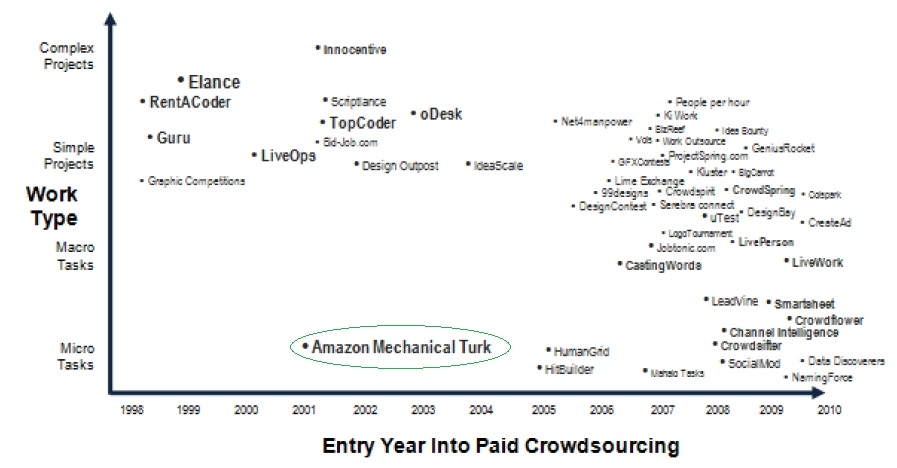
\includegraphics[width=4in]{images/history_of_crowdsourcing.jpg}
\caption{Crowdsourcing history (Frei, 2009)}
\end{figure}

\end{frame}
%%%%%%%%%%%%%%%%%%%%%%%%%%%%%%%%%%%%%%%%%%%


%%%%%%%%%%%%%%%%%%%%%%%%%%%%%%%%%%%%%%%%%%%
\begin{frame}\frametitle{A Typical Industry Task on MTurk}

Tasks are dubbed \qu{Human Intelligence Tasks} or HITs for short. Note the requester is a crowdsourcing intermediary.

\centeredimage{4.6}{typical_hit.jpg}

Note the qualifications, short description, keywords, time allotted, expiration, reward, number available.

\end{frame}
%%%%%%%%%%%%%%%%%%%%%%%%%%%%%%%%%%%%%%%%%%%

%%%%%%%%%%%%%%%%%%%%%%%%%%%%%%%%%%%%%%%%%%%
\begin{frame}\frametitle{The Turker Perspective}

\centeredimage{4.3}{typical_hit_task_page.jpg}

\end{frame}
%%%%%%%%%%%%%%%%%%%%%%%%%%%%%%%%%%%%%%%%%%%

%%%%%%%%%%%%%%%%%%%%%%%%%%%%%%%%%%%%%%%%%%%
\begin{frame}\frametitle{Turker Tools}

\centering
turkopticon.com, mturkforum.com, turkalert.com, turkrequesters blog, etc

\vspace{-0.5cm}
\centeredimage{4.6}{typical_hit_turkopticon.jpg}
\vspace{-0.3cm}
\centeredimage{3}{turkopticon_example.jpg}

\end{frame}
%%%%%%%%%%%%%%%%%%%%%%%%%%%%%%%%%%%%%%%%%%%

%%%%%%%%%%%%%%%%%%%%%%%%%%%%%%%%%%%%%%%%%%%
\begin{frame}\frametitle{The Requester Perspective}

\centeredimage{2.2}{requester_csv_file.jpg}

\vspace{-0.3cm}
\begin{itemize}
\item A spreadsheet CSV file --- each row is one HIT. \pause
\item \# rows: large, done in parallel. \pause
\item Task creation is done through a simple system or through an iframe (explained in detail later).
\end{itemize}

\end{frame}
%%%%%%%%%%%%%%%%%%%%%%%%%%%%%%%%%%%%%%%%%%%

%%%%%%%%%%%%%%%%%%%%%%%%%%%%%%%%%%%%%%%%%%%
\begin{frame}\frametitle{What is available to a Turker?}

From MTurk-tracker.com (Ipeirotis, 2010)

\vspace{-0.2cm}
\centeredimage{3.4}{mturk_hits_and_rewards.jpg}
\vspace{-0.6cm}
\centeredimage{1.7}{mturk_projects.jpg}

\end{frame}
%%%%%%%%%%%%%%%%%%%%%%%%%%%%%%%%%%%%%%%%%%%

%%%%%%%%%%%%%%%%%%%%%%%%%%%%%%%%%%%%%%%%%%%
\begin{frame}\frametitle{How many workers are there?}
\pause 
\centering

Amazon released this number in 2011: \\
$\approx$ half million registered users in 190 countries.  \pause

\centeredimage{3.4}{turkers_in_usa.jpg}

The rough distribution of Turker locations in the United States. How regular are the Turkers? Unknown.

\end{frame}
%%%%%%%%%%%%%%%%%%%%%%%%%%%%%%%%%%%%%%%%%%%

%%%%%%%%%%%%%%%%%%%%%%%%%%%%%%%%%%%%%%%%%%%
\begin{frame}\frametitle{Who are these workers?}

As of 2010, about 50\% USA, 40\% India, 10\% everywhere else (Ipeirotis, 2010a).  \pause Workers in USA and India are paid in local currency but all others are paid in gift certificates.  \pause International usage has been growing since 2010 but there has not been an updated published survey. \pause

\centeredimage{3.4}{mturk_gender.jpg} 



\end{frame}
%%%%%%%%%%%%%%%%%%%%%%%%%%%%%%%%%%%%%%%%%%%

%%%%%%%%%%%%%%%%%%%%%%%%%%%%%%%%%%%%%%%%%%%
\begin{frame}\frametitle{Who are these workers?}

\centeredimage{4.5}{mturk_age.jpg}

\centering
(Indian workers shifted younger)

\end{frame}
%%%%%%%%%%%%%%%%%%%%%%%%%%%%%%%%%%%%%%%%%%%

%%%%%%%%%%%%%%%%%%%%%%%%%%%%%%%%%%%%%%%%%%%
\begin{frame}\frametitle{Who are these workers?}

\centeredimage{4.5}{mturk_education_level.jpg}

\end{frame}
%%%%%%%%%%%%%%%%%%%%%%%%%%%%%%%%%%%%%%%%%%%

%%%%%%%%%%%%%%%%%%%%%%%%%%%%%%%%%%%%%%%%%%%
\begin{frame}\frametitle{Who are these workers?}

\centeredimage{2.5}{mturk_income.jpg}

\end{frame}
%%%%%%%%%%%%%%%%%%%%%%%%%%%%%%%%%%%%%%%%%%%

%%%%%%%%%%%%%%%%%%%%%%%%%%%%%%%%%%%%%%%%%%%
\begin{frame}\frametitle{Who are these workers?}

\centeredimage{3}{mturk_hits_per_week.jpg}
\centering
(America and India)

\end{frame}
%%%%%%%%%%%%%%%%%%%%%%%%%%%%%%%%%%%%%%%%%%%

%%%%%%%%%%%%%%%%%%%%%%%%%%%%%%%%%%%%%%%%%%%
\begin{frame}\frametitle{Who are these workers?}

\centeredimage{2.7}{mturk_secondary_source_income.jpg} \pause

\small

\vspace{-0.2cm}
Undisplayed results: about 30\% of Turkers use MTurk just to \qu{kill time,} 41\% use it for \qu{entertainment,} \pause about 15\% use it as a primary source of income (25\% in India), about 30\% are unemployed or part-time employed. \pause
\vspace{0.2cm}

Summary: 60\% say it's a good way to earn money, 70\% think it's a good way to burn time.

\end{frame}
%%%%%%%%%%%%%%%%%%%%%%%%%%%%%%%%%%%%%%%%%%%

%%%%%%%%%%%%%%%%%%%%%%%%%%%%%%%%%%%%%%%%%%%
\begin{frame}\frametitle{Types of tasks}

Top requesters (save intermediaries) taken from mturk-tracker.com July 4 - July 11, 2013 (Ipeirotis, 2010) have the following tasks categories:

\begin{table}
\begin{tabular}{cc}
Type & Estimated Proportion \\ \hline \pause
Web scouring & 42\% \\ \pause
Images related & 22\% \\ \pause
Text related \& OCR & 17\% \\ \pause
Audio related & 14\% \\ \pause
Video related & 3\% \\ \pause
Testing / Quality Assurance & 3\% \\
\end{tabular}
\end{table}

\end{frame}
%%%%%%%%%%%%%%%%%%%%%%%%%%%%%%%%%%%%%%%%%%%

%%%%%%%%%%%%%%%%%%%%%%%%%%%%%%%%%%%%%%%%%%%
\begin{frame}\frametitle{Web Scouring}

\begin{itemize} %15
\item Verify a restaurant listing
\item Match my products to Amazon products
\item Is this a web page? Easily decide if the image is a webpage.
\item Find Official Government Websites for Places
\item Find the Email addresses for wedding venues
\item Find the school website and locate the current school supply list
\item Find Yelp Reviews for Businesses
\item Categorize a Twitter search query
\item Locate company website
\item Find a company name from an email domain
\item Find main title, subtitle, and authors for a book
\item Web Page Categorization
\item Find the Official Social Media Accounts for a Website
\item Find the contact details of this Youtube channel owner.
\item Product Search Results Validation
\end{itemize}

\end{frame}
%%%%%%%%%%%%%%%%%%%%%%%%%%%%%%%%%%%%%%%%%%%

%%%%%%%%%%%%%%%%%%%%%%%%%%%%%%%%%%%%%%%%%%%
\begin{frame}\frametitle{Images related}

\begin{itemize} %8
\item Select images from a piece of adult content
\item Choose all the options this category belongs under (Amazon)
\item Label simple images
\item Categorize ad images
\item Find the bird in each image (research: Columbia)
\item Name the color of this rug
\item Estimate the age of the person in the image
\item Clickable Image Tagging
\end{itemize}

\end{frame}
%%%%%%%%%%%%%%%%%%%%%%%%%%%%%%%%%%%%%%%%%%%

%%%%%%%%%%%%%%%%%%%%%%%%%%%%%%%%%%%%%%%%%%%
\begin{frame}\frametitle{Text related / OCR}

\begin{itemize} %6
\item Judge the quality of similar sentences (research: CC Burch, UPenn)
\item Word Alignment (research: CC Burch, UPenn)
\item Categorizing buying behaviour on twitter
\item Please transcribe the following words from image
\item Classify Messages about Nissan
\item Data Transcription from a PDF
\end{itemize}

\end{frame}
%%%%%%%%%%%%%%%%%%%%%%%%%%%%%%%%%%%%%%%%%%%

%%%%%%%%%%%%%%%%%%%%%%%%%%%%%%%%%%%%%%%%%%%
\begin{frame}\frametitle{Audio related}

\begin{itemize} %5
\item Transcribe a $\approx$10sec Audio Clip
\item Transcribe Recording 
\item record a word or phrase in your own voice (research, unknown)
\item Audio transcription
\end{itemize}

\end{frame}
%%%%%%%%%%%%%%%%%%%%%%%%%%%%%%%%%%%%%%%%%%%

%%%%%%%%%%%%%%%%%%%%%%%%%%%%%%%%%%%%%%%%%%%
\begin{frame}\frametitle{Video related, Product testing}

\begin{itemize} %1
\item Watch Video Snippets and Tell Us about the Tags
\end{itemize}

\noindent\rule{10cm}{0.4pt}

\begin{itemize} %1
\item Test an automated tourist information service
\end{itemize}

\end{frame}
%%%%%%%%%%%%%%%%%%%%%%%%%%%%%%%%%%%%%%%%%%%

%%%%%%%%%%%%%%%%%%%%%%%%%%%%%%%%%%%%%%%%%%%
\begin{frame}\frametitle{MTurk and Academia}

\centeredimage{4.3}{num_pubs.pdf} 

\vspace{-0.5cm}
\centering
Explosive Growth over the past few years!

\end{frame}
%%%%%%%%%%%%%%%%%%%%%%%%%%%%%%%%%%%%%%%%%%%

%%%%%%%%%%%%%%%%%%%%%%%%%%%%%%%%%%%%%%%%%%%
\begin{frame}\frametitle{What do researchers use MTurk for?}
 \pause
\small

\ingreen{The goal of this tutorial is to teach you how to analyze data for these \qu{main uses:}}

\vspace{-0.2cm}
\begin{itemize}

\item Collecting survey responses \pause
\item Collecting labels (sometimes for building a machine learning system) \pause
\vspace{-0.5cm}
\begin{itemize}
\item Solving the \qu{noisy labeler} problem: multiple workers \pause
\item Computational linguistics: translation, document relevance, word-sense disambiguation \pause
\item Image analysis: trace objects, detect 3d planes, object similarity rating \pause
\item Audio: classify musical melodies \pause
\end{itemize}
\item Running randomized controlled experiments testing an economic, behavioral, or psychological hypothesis of interest \pause
\end{itemize}

\vspace{-0.15cm}
Other uses:
\vspace{-0.15cm}
\begin{itemize}
\item Studying MTurk from an Economic and Sociological Perspective \pause
\item Creative extensions to MTurk and plugins to MTurk (mostly computer scientists)
\end{itemize}



\end{frame}
%%%%%%%%%%%%%%%%%%%%%%%%%%%%%%%%%%%%%%%%%%%

%%%%%%%%%%%%%%%%%%%%%%%%%%%%%%%%%%%%%%%%%%%
\begin{frame}\frametitle{The three MTurk applications we will focus on}

\begin{minipage}{0.44\linewidth}
\centering

\onslide<1->{
Surveys 

\centeredimage{1}{surveys.png}
}
\onslide<2->{
Labelings 

\centeredimage{1.7}{labelings.jpg}
}
\end{minipage}
% do not remove this comment - it will displace the two minipages
\begin{minipage}{0.44\linewidth}
\centering
\onslide<3>{
Experiments

\centeredimage{1.5}{mad_scientist.jpg}
 }

\end{minipage}

\end{frame}
%%%%%%%%%%%%%%%%%%%%%%%%%%%%%%%%%%%%%%%%%%%

%%%%%%%%%%%%%%%%%%%%%%%%%%%%%%%%%%%%%%%%%%%
\begin{frame}\frametitle{The Market: HIT Completion Times}

\centeredimage{2}{hit_completion_times.jpg}
\centering
(Ipeirotis, 2010c) \\
\vspace{0.5cm} \pause
Design implications?

\end{frame}
%%%%%%%%%%%%%%%%%%%%%%%%%%%%%%%%%%%%%%%%%%%

%%%%%%%%%%%%%%%%%%%%%%%%%%%%%%%%%%%%%%%%%%%
\begin{frame}\frametitle{The Market: HIT Wages}

\centeredimage{2.5}{hit_prices.jpg} \pause

\centering
\small
There is no magic formula for HIT wage, time to completion, etc. It's all experienced trial and error. \qu{MTurk is not a M/M/1 queue.}

\end{frame}
%%%%%%%%%%%%%%%%%%%%%%%%%%%%%%%%%%%%%%%%%%%

%%%%%%%%%%%%%%%%%%%%%%%%%%%%%%%%%%%%%%%%%%%
\begin{frame}\frametitle{Microlabor Incentives}

Traditional economic theory: higher wage $\Rightarrow$ higher performance.  \pause Large body of research in economics and psychology that shows this isn't the case, and not only on MTurk.  \pause Workers must have \textit{intrinsic motivation} - which are built through non-pecuniary incentives.

\begin{itemize}
\item Mason and Watts (2010) showed that paying more results in higher \textit{volume} of work but not higher \textit{quality}. \pause
\item Many other crowdsourcing platforms e.g. galaxyzoo (classify galaxies in photographs), duolingo (translate and learn) motivate by providing an educational experience.
\end{itemize}

\end{frame}
%%%%%%%%%%%%%%%%%%%%%%%%%%%%%%%%%%%%%%%%%%%

%%%%%%%%%%%%%%%%%%%%%%%%%%%%%%%%%%%%%%%%%%%
\begin{frame}\frametitle{Microlabor Incentives}

\begin{itemize}
\item Chandler and Kapelner (2013) found that increasing \qu{meaningfulness} of a task will increase participation and quantity but not quality. To decrease quality, the worker had to be convinced their work would \textit{never} be looked at. \pause
\item \qu{Gamification} is a new, hot field! \pause Making the task fun via create leaderboards, collections, point systems, earning credit, skill level-ups (like a video game), timed response makes a big difference. Horton and Chilton (2010) found workers to be  \qu{target earners} who stop after reaching some predetermined goal (e.g. exactly \$1).  \pause
\end{itemize}

Not so relevant for surveys, \textit{small} labeling tasks, or randomized experiments, but very useful for massive crowdsourced projects.

\end{frame}
%%%%%%%%%%%%%%%%%%%%%%%%%%%%%%%%%%%%%%%%%%%

%%%%%%%%%%%%%%%%%%%%%%%%%%%%%%%%%%%%%%%%%%%
\begin{frame}\frametitle{Ethical Dilemmas}

\begin{itemize}
\item In our experience, we've measured hourly wages at about \$1.12/hr (Chandler and Kapelner, 2013) and Chilton (2010) measured the reservation wage at \$1.38/hr (both \textit{pretax}).  \pause These estimates are substantially under minimum wage and the Turkers receive zero benefits.  \pause Is this a \qu{new digital sweatshop} that Harvard law professor Zittrain claims? \pause
\item Turkers are at the whim of requesters who get to veto their work, at times dishonestly, and they do not get paid. \pause
\item Requesters are under no obligation to inform the Turker of the meaning / purpose of the HITs. Turkers could be \textit{deceived} into contributing to something they find personally unethical without their knowledge. (We will talk about Institutional Review Board stuff later).
\end{itemize}

\end{frame}
%%%%%%%%%%%%%%%%%%%%%%%%%%%%%%%%%%%%%%%%%%%

%%%%%%%%%%%%%%%%%%%%%%%%%%%%%%%%%%%%%%%%%%%
\begin{frame}\frametitle{Ethical Dilemmas}
\pause

\begin{itemize}
\item MTurk is considered the \qu{wild west} by some in the legal community: no governmental regulation to date (age? max hours? unionization rights?) \pause
\item Should human mental cycles be an \qu{undifferentiated commodity} without regulation? \pause
\end{itemize}

\centering
\scriptsize
for more information see: \\
Horton (2011a), Kittur et al (2013), Zittrain (2008), Felstiner (2010)


\end{frame}
%%%%%%%%%%%%%%%%%%%%%%%%%%%%%%%%%%%%%%%%%%%

%%%%%%%%%%%%%%%%%%%%%%%%%%%%%%%%%%%%%%%%%%%
\begin{frame}\frametitle{Checkpoint}

We've covered:

\begin{itemize}
\item crowdsourcing \pause
\item microlabor on MTurk: what it looks like, how it's created  \pause
\item MTurk labor market: requesters and Turkers \pause
\item how industry and academia make use of MTurk \pause
\end{itemize}

\begin{block}{Goal A Complete}
\small
Know what MTurk is used for in academics and industry \textit{and thereby} recognize where crowdsourcing could be useful in your work
\end{block}

\end{frame}
%%%%%%%%%%%%%%%%%%%%%%%%%%%%%%%%%%%%%%%%%%%

\section{Survey Research}

%%%%%%%%%%%%%%%%%%%%%%%%%%%%%%%%%%%%%%%%%%%
\begin{frame}\frametitle{Surveys}

\centeredimage{1}{surveys.png}

\end{frame}
%%%%%%%%%%%%%%%%%%%%%%%%%%%%%%%%%%%%%%%%%%%

%%%%%%%%%%%%%%%%%%%%%%%%%%%%%%%%%%%%%%%%%%%
\begin{frame}\frametitle{Surveying on MTurk}

\centeredimage{3}{typical_survey.jpg}

Surveys are one of the most common tasks on MTurk for \textit{both} industry and research.

\end{frame}
%%%%%%%%%%%%%%%%%%%%%%%%%%%%%%%%%%%%%%%%%%%

%%%%%%%%%%%%%%%%%%%%%%%%%%%%%%%%%%%%%%%%%%%
\begin{frame}\frametitle{Survey Validity}
\small
The main issue in survey research is whether the survey properly reflects the population of interest. Political scientists Berinsky et al (2012) asks this question for the US population. They find the following:

\centeredimage{1.9}{mturk_US_pop_educ_age_income.jpg}

\end{frame}
%%%%%%%%%%%%%%%%%%%%%%%%%%%%%%%%%%%%%%%%%%%

%%%%%%%%%%%%%%%%%%%%%%%%%%%%%%%%%%%%%%%%%%%
\begin{frame}\frametitle{Survey Validity}

\centeredimage{1.8}{mturk_US_pop_ideology.jpg}

\end{frame}
%%%%%%%%%%%%%%%%%%%%%%%%%%%%%%%%%%%%%%%%%%%

%%%%%%%%%%%%%%%%%%%%%%%%%%%%%%%%%%%%%%%%%%%
\begin{frame}\frametitle{Survey Validity}

They also studied whether or not Turkers were \qu{chronic survey-takers} and found over 4 months, of $\approx$ 1600 unique Turkers, 70\% took only one survey. Hence there probably is a small effect of \textit{cross-survey stimuli}. \pause

\vspace{0.2cm}

Conclusions: the Turkers are younger, more politically liberal, slightly less wealthy, slightly more educated, enjoy cognitively-demanding tasks slightly more than gold standard probability samples of Americans. \pause

\vspace{0.2cm}

Thus, for survey research, you can build stratified samples.

\end{frame}
%%%%%%%%%%%%%%%%%%%%%%%%%%%%%%%%%%%%%%%%%%%

%%%%%%%%%%%%%%%%%%%%%%%%%%%%%%%%%%%%%%%%%%%
\begin{frame}\frametitle{Problems with collecting surveys}
\pause

\small

Many respondents \qu{cheat} or are lazy when filling out these surveys (see Krosnick, 2000). \pause There are four steps: interpretation of question, \pause retrieval of information, \pause judging retrieved information, \pause and interpreting and selecting a response. \pause
Expending the minimum amount of effort to complete the survey may involve skipping some of these steps. \pause

Other survey design problems observed: \pause

\begin{itemize}
\item Response order: more likely to fill out the first or last response on a multiple response question, thus, randomize! \pause
\item Acquiescence bias: more likely say  \qu{agree / true / yes} with the surveyor than \qu{disagree / false / no,} thus, avoid these questions! \pause
\item No opinion filter: more likely to pick the \qu{no opinion} or \qu{don't know} option if given the opportunity, don't give it! \pause
\item Rankings inaccuracy: ranking many items puts undue stress on the survey-taker, thus ratings are recommended \pause
\end{itemize}

Krosnick recommends \textbf{minimizing task difficulty} and \textbf{maximizing subject motivation}.

\end{frame}
%%%%%%%%%%%%%%%%%%%%%%%%%%%%%%%%%%%%%%%%%%%

%%%%%%%%%%%%%%%%%%%%%%%%%%%%%%%%%%%%%%%%%%%
\begin{frame}\frametitle{A way to mitigate satisficing}

Kapelner and Chandler (2010) recommend fading in each word... \pause

\begin{figure}[htp]
\centering
\includemovie[autoplay, poster=images/imc.jpg]{2.875in}{2.3in}{images/kapcha.mpg}
\end{figure}
\centering \small
The \qu{IMC}

\end{frame}
%%%%%%%%%%%%%%%%%%%%%%%%%%%%%%%%%%%%%%%%%%%

%%%%%%%%%%%%%%%%%%%%%%%%%%%%%%%%%%%%%%%%%%%
\begin{frame}\frametitle{Fade-in results}

\only<1>{
\centeredimage{3}{results_imc_question.jpg}
}
\only<2>{
\centeredimage{4.5}{table_6_kapcha_paper.jpg}
}
\end{frame}
%%%%%%%%%%%%%%%%%%%%%%%%%%%%%%%%%%%%%%%%%%%

%%%%%%%%%%%%%%%%%%%%%%%%%%%%%%%%%%%%%%%%%%%
\begin{frame}\frametitle{MTurkers found to beat Ivy-leaguers}

\centeredimage{3.5}{mturkers_good.jpg}

\centering
IMC pass rate by subpopulation

\end{frame}
%%%%%%%%%%%%%%%%%%%%%%%%%%%%%%%%%%%%%%%%%%%

%%%%%%%%%%%%%%%%%%%%%%%%%%%%%%%%%%%%%%%%%%%
\begin{frame}\frametitle{MTurk Survey Studies}
 \pause

\footnotesize
\vspace{-0.2cm}
\begin{itemize}
\footnotesize

\item Finding: Childhood socioeconomic status influences subject likelihood to \qu{diversify} and hedge their bets (White et al, 2013) \pause
\item What do terms like \qu{unlikely} and \qu{improbable} mean to people mathematically? (Teigen et al., 2013) \pause
\item How \qu{quickly} do people perceive life has changed is changing, and will change for different age groups to investigate the \qu{end of history illusion.} (Quoidbach et al., 2013) \pause
\item Ascertain levels of narcissism, psychopathy and Machiavellianism to test the validity of psychological models. (Jonason and Luevano, 2013) \pause
\item Measure \qu{intolerance} differences between  those leaning politically left and right (Crawford and Pilansky, 2013)  \pause
\item See if medical pictograms (e.g. \qu{take pill with food}) are understandable (Yu et al, 2013).
\end{itemize}

\vspace{-0.5cm}
\centeredimage{2.5}{pictograms.jpg}

\end{frame}
%%%%%%%%%%%%%%%%%%%%%%%%%%%%%%%%%%%%%%%%%%%

%%%%%%%%%%%%%%%%%%%%%%%%%%%%%%%%%%%%%%%%%%%
\begin{frame}\frametitle{Checkpoint}

We've covered: \pause

\begin{itemize}
\item validity / stratified sampling on MTurk \pause
\item understanding satisficing issues on MTurk and apply it to design \pause
\item a quick review of survey research on MTurk \pause
\end{itemize}

\begin{block}{Goal B Complete}
\small
Use MTurk for survey research
\end{block}

\end{frame}
%%%%%%%%%%%%%%%%%%%%%%%%%%%%%%%%%%%%%%%%%%%

\section{Labeling and Machine Learning}

%%%%%%%%%%%%%%%%%%%%%%%%%%%%%%%%%%%%%%%%%%%
\begin{frame}\frametitle{Labeling and Machine Learning}

\centeredimage{1.7}{labelings.jpg}

\end{frame}
%%%%%%%%%%%%%%%%%%%%%%%%%%%%%%%%%%%%%%%%%%%

%%%%%%%%%%%%%%%%%%%%%%%%%%%%%%%%%%%%%%%%%%%                                                                                                  
\begin{frame}\frametitle{Crowdsourcing for labeling}

\begin{itemize}
\item The first widely used application
\item Often machine vision or language
\begin{itemize}
\item Objects in images (or their features)
\item Word or document sense, sentiment, translation, ...
\item Audio transcription
\end{itemize}
\end{itemize}

Collection often goes beyond labels: proposed translation or summary

\end{frame}
%%%%%%%%%%%%%%%%%%%%%%%%%%%%%%%%%%%%%%%%%%%                                                                                                  
\begin{frame}\frametitle{The labeling process}

\begin{itemize}
  \item Define task and make instructions
\begin{itemize}
  \item HITs are usually fast and simple
\end{itemize}
  \item Pretest in-house and refine instructions
  \item Get IRB approval or exemption
  \item Decide on collection process
       \begin{itemize}
        \item How to select items to label?
        \item How many labels?
        \item Batch or adaptive item selection?
      \end{itemize}
  \item Code M-turk application
  \item Collect data
  \item Screen for spammers
  \item Estimate model
\end{itemize}

\end{frame}

%%%%%%%%%%%%%%%%%%%%%%%%%%%%%%%%%%%%%%%%%%%                                                                                                  
\begin{frame}\frametitle{Test HITS in-house}

\begin{itemize}
  \item What is confusing?
  \item How high is inter-annotator agreement?
  \item Refine instructions
\end{itemize}

{\bf How positive or negative or negative is the sentiment?}

\vspace{0.2cm}

``I just bought a Corrolla''

\vspace{0.1cm}

``I like my friends but their driving me crazy''

\end{frame}
%%%%%%%%%%%%%%%%%%%%%%%%%%%%%%%%%%%%%%%%%%%                                                                                                  
\begin{frame}\frametitle{Get IRB approval}

\begin{itemize}
  \item Institutional Review Board (IRB) approval or exemption
  \item Takes longer than you think
  \item Inconsistent across schools
  \item Big issue: privacy
  \item Usually expedited due to being exempt under category \#2
\end{itemize}

\end{frame}

%%%%%%%%%%%%%%%%%%%%%%%%%%%%%%%%%%%%%%%%%%%                                                                                                  
\begin{frame}\frametitle{Code M-turk application}

\begin{itemize}
  \item How hard is it?
 \begin{itemize}
    \item a couple programmer weeks to modify existing code to a new task
 \end{itemize}
  \item What code exists to do this already?
  \item Gotchas?
\end{itemize}

\end{frame}

%%%%%%%%%%%%%%%%%%%%%%%%%%%%%%%%%%%%%%%%%%%                                                                                                  
\begin{frame}\frametitle{Screen for spammers}

\begin{itemize}
  \item Not a problem in our experience -- but others have different experiences
  \item Single turker methods
      \begin{itemize}
        \item speed, variety, accuracy
      \end{itemize}
  \item Agreement with other annotators
\end{itemize}

\end{frame}
%%%%%%%%%%%%%%%%%%%%%%%%%%%%%%%%%%%%%%%%%%%                                                                                                  

%%%%%%%%%%%%%%%%%%%%%%%%%%%%%%%%%%%%%%%%%%%
\begin{frame}\frametitle{Case Study: Word Sense Disambiguation}

\qu{The level of good-faith participation by Turkers is surprisingly high, given the generally small nature of the payment.} (Callison-Burch, 2009)


\begin{thebibliography}{1}
\bibitem{kap2}
\tiny
Kapelner, A, Kaliannan, K, Schwartz, A, Ungar, L, Foster, D,  New Insights from Coarse Word Sense Disambiguation in the Crowd In Proceedings of CoLING, 2012, pp539--548
\end{thebibliography} \pause

\vspace{0.5cm}

\textbf{What is Word Sense Disambiguation? (WSD)} \\

\vspace{0.2cm}

Language is ambiguous and many words can denote different ``meanings''

\begin{itemize}
\item I can hear \textit{bass} sounds.
\item They like grilled \textit{bass}.
\end{itemize}

WSD has been described as ``AI-complete'' which means it is equivalent to solving central problems in artificial intelligence \ala the Turing Test.

\end{frame}
%%%%%%%%%%%%%%%%%%%%%%%%%%%%%%%%%%%%%%%%%%%

%%%%%%%%%%%%%%%%%%%%%%%%%%%%%%%%%%%%%%%%%%%
\begin{frame}\frametitle{Our HIT: the WSD labeling task}

\begin{columns}
\begin{column}{.5\textwidth}
\centering
\centeredimage{2.2}{our_hit.jpg}
\end{column}
\begin{column}{.5\textwidth}
\scriptsize
\begin{itemize}
\scriptsize
\item A subset of the Penn Treebank Wall Street Journal Corpus
\item A collapsed version of Wordnet 2.1
\item Nouns and verbs only
\end{itemize}

\vspace{0.2cm}

This data is from the ``OntoNotes'' project (2006). They iteratively make the senses more and more ``coarse-grained'' until they achieve a 90\% ITA among the annotators. For example, the word ``share:'' \\

\vspace{0.2cm}

One snippet, one word, all coarse senses. Optional feedback box. Prevent cheating / satisficing by (1) fading in the words slowly (2) randomly ordering the senses.

\vspace{0.2cm}

1,000 words, each disambiguated by 10 Turkers each

\end{column}
\end{columns}

\end{frame}
%%%%%%%%%%%%%%%%%%%%%%%%%%%%%%%%%%%%%%%%%%%

%%%%%%%%%%%%%%%%%%%%%%%%%%%%%%%%%%%%%%%%%%%
\begin{frame}\frametitle{The Data and the questions we want to answer}

595 Turkers, 10,000 HITs at 10\cent~ each \\

total time: 51hr --- throughput: \ingreen{4700 labels / day} with cost: \$110.\\

Krippendorf's $\alpha = 0.66$ which is fair interrater reliability.

\vspace{0.2cm}

{\bf We tried to answer the following in data analysis:}

\begin{itemize}
\item Can we combine Turker responses to boost accuracy?
\item Is the workers' performance heterogeneous?
\item Which features in the target word, the snippet text, and the text of the sense choices affect accuracy?
\item Which characteristics in the Turker's engagement of the task affect accuracy?
\end{itemize}

Today: the first two goals.

\end{frame}
%%%%%%%%%%%%%%%%%%%%%%%%%%%%%%%%%%%%%%%%%%%

%%%%%%%%%%%%%%%%%%%%%%%%%%%%%%%%%%%%%%%%%%%
\begin{frame}\frametitle{Boosting Accuracy}

{\bf Can we combine Turker responses naively to boost accuracy?} \\
\vspace{0.5cm}

Combine annotations and use plurality vote arbitrating ties randomly:

\begin{table}[htp]
\centering
\footnotesize
\begin{tabular}{l|ccccccccc|c}
\# of Dis & 2 & 3 & 4 & 5 & 6 & 7 & 8 & 9 & 10 & 2.4 (1st pl)\\
\hline
Accuracy & .73 & .80 & .81 & .82 & .83 & .84 & .84 & .84 & .86 & .81 \\
\end{tabular}
\end{table}

Combining 10 untrained Turkers is competitive with the accuracy of state-of-the-art algorithms.

\vspace{0.2cm}

Ipeirotis, 2011 claims that \qu{majority vote works best when workers have similar quality} and if not:
\begin{itemize}
\item Find best worker and use that label
\item Model worker quality and combine
\end{itemize}

\end{frame}
%%%%%%%%%%%%%%%%%%%%%%%%%%%%%%%%%%%%%%%%%%%

%%%%%%%%%%%%%%%%%%%%%%%%%%%%%%%%%%%%%%%%%%%
\begin{frame}\frametitle{Using labels from different-quality workers}

Dawid and Skene (1979) proposed an expectation-maximization algorithm:

\begin{enumerate}
\item[0] Initialize with the aggregate labels being the majority vote
\item[1] Estimate confusion matrix for each worker
\item[2] Estimate aggregate labels again (if gold data exists, keep it)
\item[3] Repeat steps 2-3 until convergence criteria is met
\end{enumerate}

For a bayesian version see Raykar et al (2010). 

\end{frame}
%%%%%%%%%%%%%%%%%%%%%%%%%%%%%%%%%%%%%%%%%%%

%%%%%%%%%%%%%%%%%%%%%%%%%%%%%%%%%%%%%%%%%%%
\begin{frame}\frametitle{Using labels from different-quality workers}

Ipeirotis et al (2010a) is able to tease out bias and error. For $K$ categories, cost matrix $\braces{c_{ij}}$, and soft labels $p_1, \ldots, p_K$ for a given worker,

\beqn
\text{Expected Cost}(p_1, \ldots, p_K) := \sum_{i=1}^K \sum_{j=1}^K p_i p_j c_{ij}
\eeqn

\centeredimage{3}{cost_labels.jpg}

\end{frame}
%%%%%%%%%%%%%%%%%%%%%%%%%%%%%%%%%%%%%%%%%%%

%%%%%%%%%%%%%%%%%%%%%%%%%%%%%%%%%%%%%%%%%%%
\begin{frame}\frametitle{Using labels from different-quality workers}

There are high costs when probabilities are diffuse and low costs when less diffuse. Now compute a quality score, where \qu{spammer} is defined as a discrete uniform distribution over labels:

\beqn
\text{Quality Score}(worker) := 1 - \frac{\text{Expected Cost}\parens{\text{worker}}}{\text{Expected Cost}\parens{\text{spammer}}}
\eeqn

Plug this into the EM algorithm on previous slide.

\vspace{0.5cm}

Conclusions: you may want to have some gold data when benefit of learning quality differences outweighs cost of gold data (Wang et al, 2011), try to weight workers appropriately when combining.

\end{frame}
%%%%%%%%%%%%%%%%%%%%%%%%%%%%%%%%%%%%%%%%%%%

%%%%%%%%%%%%%%%%%%%%%%%%%%%%%%%%%%%%%%%%%%%
\begin{frame}\frametitle{Are all workers the same in our task?}

Do we have spammers and superstars? Is anyone different from the average, $p_{\text{avg}} = .73$? Let $C_w$ be the number correct for Turker w.


\beqn
H_0: C_1, C_2, \ldots, C_W \inddist \binomial{n_w}{p_{\text{avg}}}
\eeqn
\vspace{-0.25cm}

\begin{columns}
\begin{column}{.5\textwidth}
\centeredimage{1.8}{spammers_and_superstars.jpg}
\end{column}
\begin{column}{.5\textwidth}
(with Bonferroni-corrected Binomial proportion CI's $\alpha = 5\%$). \\
\vspace{0.5cm}

We are forced to reject on the account of four workers. \\ To a first order approximation, all Turkers are the same. Also note: no learning effect was found (unshown).

\end{column}
\end{columns}

\end{frame}
%%%%%%%%%%%%%%%%%%%%%%%%%%%%%%%%%%%%%%%%%%%

%%%%%%%%%%%%%%%%%%%%%%%%%%%%%%%%%%%%%%%%%%%
\begin{frame}\frametitle{The Goal: Active Learning Loop}

\qu{Crowdsourcing is cheap, but not free} --- so use active learning.
\centeredimage{3}{cyborg.jpg}

Here, $\hat{S}$ is a machine learning classifier. This \qu{active
  learning} model uses $\hat{S}$ when the machine is \qu{confident}
otherwise humans. The human data is then integrated into the model,
and $\hat{S}$ improves.

\end{frame}
%%%%%%%%%%%%%%%%%%%%%%%%%%%%%%%%%%%%%%%%%%%


%%%%%%%%%%%%%%%%%%%%%%%%%%%%%%%%%%%%%%%%%%%
\begin{frame}\frametitle{Integrating MTurking with machine learning}

Tradeoff between getting \textit{higher quality} data (either via combining multiple labels or getting better Turkers) and getting \textit{more} data.

\centeredimage{3}{tradeoffs_machine_learning.jpg}
\centering
(Ipeirotis, WWW'11)

\end{frame}
%%%%%%%%%%%%%%%%%%%%%%%%%%%%%%%%%%%%%%%%%%%

%%%%%%%%%%%%%%%%%%%%%%%%%%%%%%%%%%%%%%%%%%%
\begin{frame}\frametitle{MTurk labeling data often has block structure}

\small

Building $\hat{S}$ requires a machine learning algorithm which usually expects:

\beqn
Y_i = f(x_{1i}, \ldots, x_{pi}) + \errorrv_i, \quad \errorrv_1, \ldots, \errorrv_n \iid e(0, \sigsq)
\eeqn

\begin{minipage}{0.60\linewidth}

What does data from MTurk \textit{really} look like?

\centeredimage{2.5}{crowdsourcing_data_format.jpg}

\end{minipage}
\begin{minipage}{0.38\linewidth}
\scriptsize


\vspace{-0.2cm}
\centeredimage{1.5}{eff_n_as_function_of_rho.jpg}
\vspace{-0.2cm}

Thus, $n_{\text{eff}} \in \bracks{12, 31}$, an inconvenient reality that off-the-shelf ML algorithms do not consider:\\

\vspace{-0.4cm}
\footnotesize
\beqn
\berrorrv \sim e\parens{\zerovec,~ \sigsq\threebythreemat{\D_1}{}{}{}{\ddots}{}{}{}{\D_{12}}}
\eeqn

\end{minipage}

\end{frame}
%%%%%%%%%%%%%%%%%%%%%%%%%%%%%%%%%%%%%%%%%%%

%%%%%%%%%%%%%%%%%%%%%%%%%%%%%%%%%%%%%%%%%%%
\begin{frame}\frametitle{Handling the block structure}
\vspace{-0.1cm}

\begin{itemize}
\item Non-parametric, black-box algorithms which model the classification or regression function cannot usually support a correlation structure natively.  
\item Prior work includes a vast literature in the medical domain.
\item Typical simple methods use random-effects linear models or maximum likelihood linear models ($\thetavec = \bracks{\rho, \bbeta}$). Use interactions built with your favorite model builder (stepwise, etc). For classification, you can use generalized estimating equations (Liang and Zeger, 1986).
\item More recent work uses methods like random forests for cluster-correlated data (Karpievitch et al., 2009) or random-effects expectation-maximization trees (Sela and Simonoff, 2011)
\end{itemize}

\end{frame}
%%%%%%%%%%%%%%%%%%%%%%%%%%%%%%%%%%%%%%%%%%%

%%%%%%%%%%%%%%%%%%%%%%%%%%%%%%%%%%%%%%%%%%%
\begin{frame}\frametitle{Handling the block structure}

Our best advice: ignore dependence if:

\begin{itemize}
\item you built a sophisticated linear models and test $H_0: \rho = 0$ (for random effects: $\tausq = 0$) and it fails to reject
\item your out-of-sample RMSE on gold data for the black boxes is much higher than models estimating intercepts or correlations, you may just want to ignore dependence since you're getting more juice out of the non-parametric ability of the black box.
\end{itemize}

\end{frame}
%%%%%%%%%%%%%%%%%%%%%%%%%%%%%%%%%%%%%%%%%%%

%%%%%%%%%%%%%%%%%%%%%%%%%%%%%%%%%%%%%%%%%%%
\begin{frame}\frametitle{Group Project}

\centering

Spend 5 minutes with your neighbors coming up with a labeling task that integrates with a machine learning classifier.

\centeredimage{2}{group_project.jpg}

We'll discuss feasibility of projects.

\end{frame}
%%%%%%%%%%%%%%%%%%%%%%%%%%%%%%%%%%%%%%%%%%%

%%%%%%%%%%%%%%%%%%%%%%%%%%%%%%%%%%%%%%%%%%%
\begin{frame}\frametitle{Some literature on MTurk for labeling}

\begin{itemize}
\item Classic work crowdsourcing natural language processing tasks (Snow et al., 2008)
\item Document relevance (Agrawal et al., 2009)
\item Machine translation of different languages (Callison-Burch, 2009)
\item Personality and \qu{well-being} on Facebook  (Schwartz, Kapelner, Ungar et al., 2013)
\item Similarity of different melodies (Urbano et al., 2010)
\item Transcription (Marge et al., 2010)
\item Extract medical terms from patient-written text (Maclean et al., 2013) 
\end{itemize}

\end{frame}
%%%%%%%%%%%%%%%%%%%%%%%%%%%%%%%%%%%%%%%%%%%

%%%%%%%%%%%%%%%%%%%%%%%%%%%%%%%%%%%%%%%%%%%
\begin{frame}\frametitle{Checkpoint}

We've covered:

\begin{itemize}
\item A natural language processing case study about labeling on MTurk
\item Handling noisy / biased labels
\item Using data to create a machine learning classifier
\item Handling label dependence due to worker portfolios
\end{itemize}

\begin{block}{Goal C Complete}
\small
\begin{enumerate}
\item[C] For crowdsourced labeling tasks:
\begin{enumerate}[1]
\item Evaluate if the labeling task is suitable for crowdsourcing
\item Design the labeling task
\item Analyze the resulting data
\end{enumerate}
\end{enumerate}
\end{block}

\end{frame}
%%%%%%%%%%%%%%%%%%%%%%%%%%%%%%%%%%%%%%%%%%%


\section{Randomized Experiments}

%%%%%%%%%%%%%%%%%%%%%%%%%%%%%%%%%%%%%%%%%%%
\begin{frame}\frametitle{Experiments}

\centeredimage{1}{mad_scientist.jpg}

\end{frame}
%%%%%%%%%%%%%%%%%%%%%%%%%%%%%%%%%%%%%%%%%%%

%%%%%%%%%%%%%%%%%%%%%%%%%%%%%%%%%%%%%%%%%%%
\begin{frame}\frametitle{Case Study}
\scriptsize 

\qu{Conduct a wide range of experiments involving potentially large numbers of participants (hundreds or even thousands, but probably not millions) quickly and cheaply} - Mason and Watts (2010) \pause

\begin{thebibliography}{1}
\bibitem{kap}
\tiny
Chandler, D. and Kapelner, A. Breaking Monotony with Meaning: Motivation in Crowdsourcing Markets, Journal of Economic Behavior \& Organization 90, 123-133, 2013
\end{thebibliography}

\scriptsize 
\vspace{0.2cm}
Study testing the effect of \qu{meaningfulness} on three outcome measures: labor supply, work quantity and work quality. \\ \pause

\centeredimage{1.3}{basic_meaning_task.jpg}
\scriptsize
Directions: click on ``tumor cells'' / ''objects of interest.'' \pause Experiment run in US and India for comparison. 

\vspace{-0.2cm}
\centeredimage{0.8}{usa_vs_india.jpg}

\end{frame}
%%%%%%%%%%%%%%%%%%%%%%%%%%%%%%%%%%%%%%%%%%%

%%%%%%%%%%%%%%%%%%%%%%%%%%%%%%%%%%%%%%%%%%%
\begin{frame}\frametitle{Treatments and Hypotheses}

Three experimental treatments: \pause

\begin{itemize}
\item \textit{meaningful} treatment: Turkers were told that they were helping cancer researchers mark tumor cells in medical images \pause
\item \textit{zero-context} treatment: Turkers were told to mark \qu{objects of interest} in images \pause
\item \textit{shredded} treatment: Turkers were told to mark \qu{objects of interest} in images \textit{and} their labelings will be discarded upon submission \pause
\end{itemize}

Hypotheses: Monotonically with \textit{meaningfulness}, more workers will... \pause

\begin{itemize}
\item ``show up'' (\ie the labor supply increases) \pause
\item work longer (\ie on more images) \pause
\item work more accurately (\ie clicking closer to the center) \pause
\end{itemize}

\scriptsize

+ Minor hypotheses about US vs. India

\end{frame}
%%%%%%%%%%%%%%%%%%%%%%%%%%%%%%%%%%%%%%%%%%%

%%%%%%%%%%%%%%%%%%%%%%%%%%%%%%%%%%%%%%%%%%%
\begin{frame}\frametitle{The HIT Listing}

\centeredimage{4}{meaning_hit_1.jpg}

Note the fake name.  \pause Old screenshot: corrections: each HIT lasted one hour only, then it was reposted. We reposted in batches of 1000 so it would appear to the Turkers that many HITs were available. 


\end{frame}
%%%%%%%%%%%%%%%%%%%%%%%%%%%%%%%%%%%%%%%%%%%

%%%%%%%%%%%%%%%%%%%%%%%%%%%%%%%%%%%%%%%%%%%
\begin{frame}\frametitle{The HIT Preview}

\centeredimage{4}{meaning_hit_2.jpg}

\end{frame}
%%%%%%%%%%%%%%%%%%%%%%%%%%%%%%%%%%%%%%%%%%%

%%%%%%%%%%%%%%%%%%%%%%%%%%%%%%%%%%%%%%%%%%%
\begin{frame}\frametitle{The pre-HIT}

\centeredimage{1.5}{colorblindness.jpg}

\scriptsize

Check demographics,  \pause eliminate spam,  \pause ensure audio works (few Turkers excluded).

\vspace{0.2cm}

Note that this was all custom-built software externally hosted using Ruby-on-Rails. This was \textit{not} built using Amazon's HIT builder tools.

\end{frame}
%%%%%%%%%%%%%%%%%%%%%%%%%%%%%%%%%%%%%%%%%%%

%%%%%%%%%%%%%%%%%%%%%%%%%%%%%%%%%%%%%%%%%%%
\begin{frame}\frametitle{Instructional Video}

Now... randomize... to M, Z, S \pause

\centeredimage{3}{training_video.jpg} \pause

\footnotesize
3min instructional video with 15 treatment cues in the video, e.g\\
\vspace{0.3cm}
\tiny
[ \inred{Your job will be to help identify tumor cells in images and we appreciate your help.} /\\
\inblue{In this task, you'll look at images and find objects of interest.}]

\end{frame}
%%%%%%%%%%%%%%%%%%%%%%%%%%%%%%%%%%%%%%%%%%%

%%%%%%%%%%%%%%%%%%%%%%%%%%%%%%%%%%%%%%%%%%%
\begin{frame}\frametitle{Instructional Video}

\centeredimage{3.5}{scientists_producing.jpg}

\end{frame}
%%%%%%%%%%%%%%%%%%%%%%%%%%%%%%%%%%%%%%%%%%%

%%%%%%%%%%%%%%%%%%%%%%%%%%%%%%%%%%%%%%%%%%%
\begin{frame}\frametitle{The \qu{Quiz}}

\centeredimage{3.5}{quiz.jpg}

\end{frame}
%%%%%%%%%%%%%%%%%%%%%%%%%%%%%%%%%%%%%%%%%%%

%%%%%%%%%%%%%%%%%%%%%%%%%%%%%%%%%%%%%%%%%%%
\begin{frame}\frametitle{The Experimental Task}

Label as many as you want at a decreasing wage scale: 10\cent, 9\cent, 8\cent, 7\cent, \ldots, 2\cent, 2\cent, 2\cent, \ldots \pause
\centeredimage{2.8}{training_for_cells.jpg}

 \pause


\vspace{-0.3cm}
\centering

\tiny This training screen is an adaptation of \texttt{DistributeEyes}, a project funded by Susan Holmes of Stanford University under NIH Grant \#R01GM086884-02.

\end{frame}
%%%%%%%%%%%%%%%%%%%%%%%%%%%%%%%%%%%%%%%%%%%

%%%%%%%%%%%%%%%%%%%%%%%%%%%%%%%%%%%%%%%%%%%
\begin{frame}\frametitle{Do Another Task?}

\centeredimage{4}{bmom_do_another_labeling.jpg}

\end{frame}
%%%%%%%%%%%%%%%%%%%%%%%%%%%%%%%%%%%%%%%%%%%

%%%%%%%%%%%%%%%%%%%%%%%%%%%%%%%%%%%%%%%%%%%
\begin{frame}\frametitle{Possible Images}

\vspace{-0.1cm}
\begin{figure}[htp]
\centering
\subfigure{
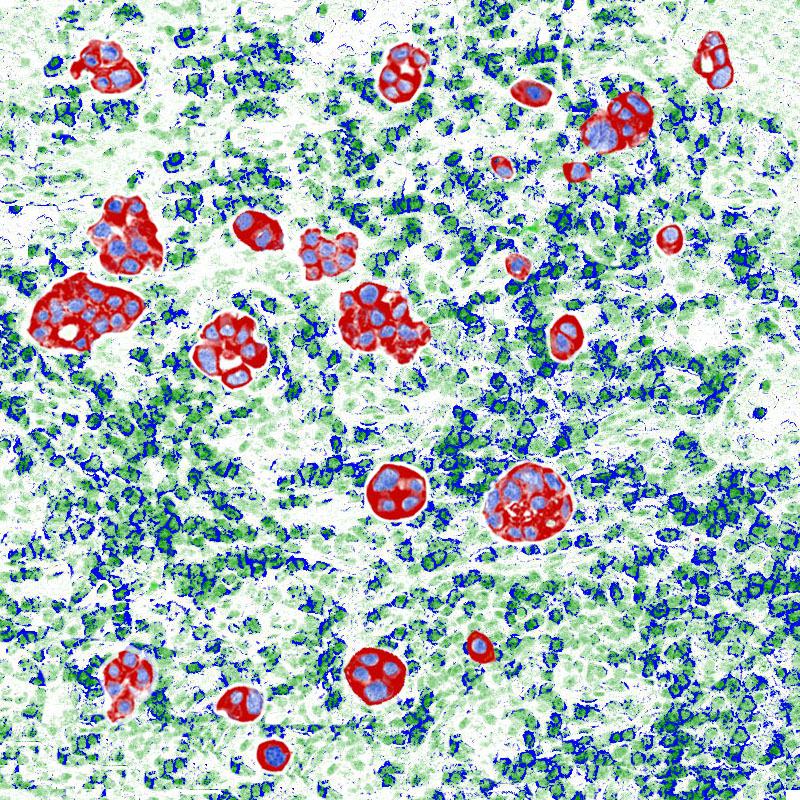
\includegraphics[width=0.8in]{images/possible_image_01.jpg}
}
\subfigure{
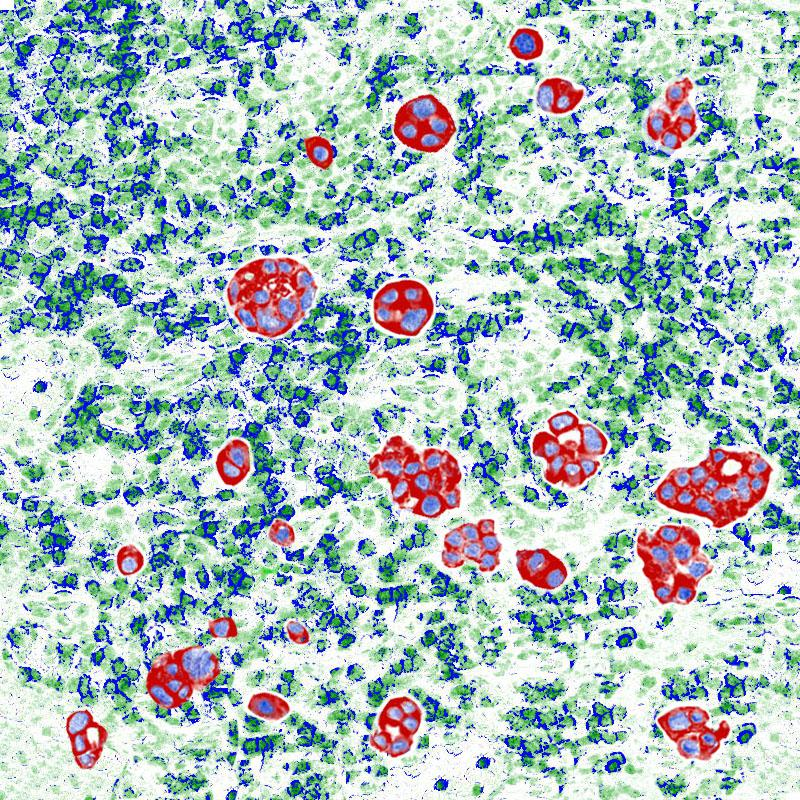
\includegraphics[width=0.8in]{images/possible_image_02.jpg}
}
\subfigure{
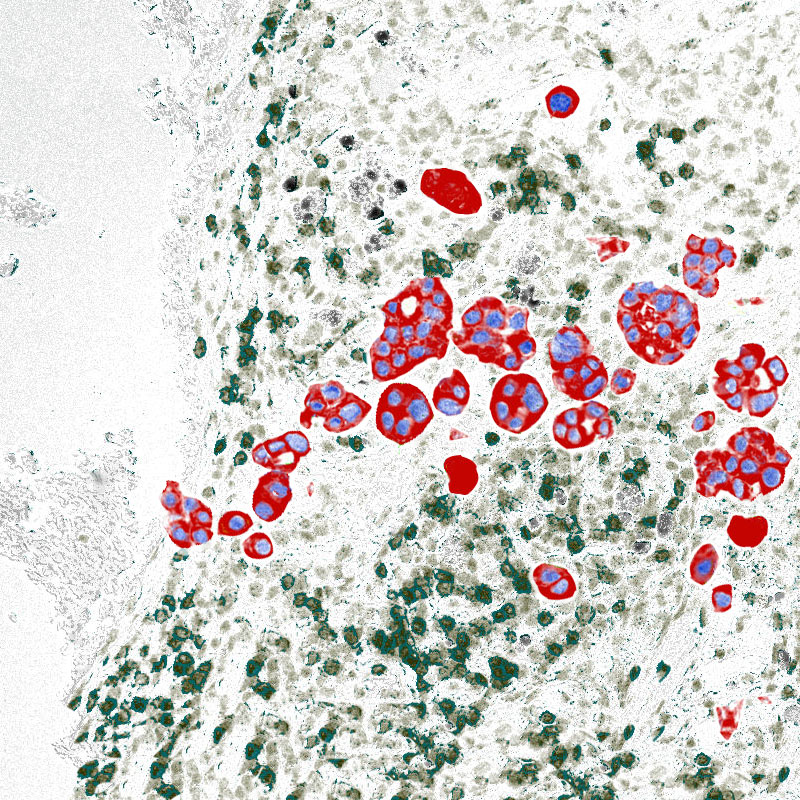
\includegraphics[width=0.8in]{images/possible_image_03.jpg}
}
\subfigure{
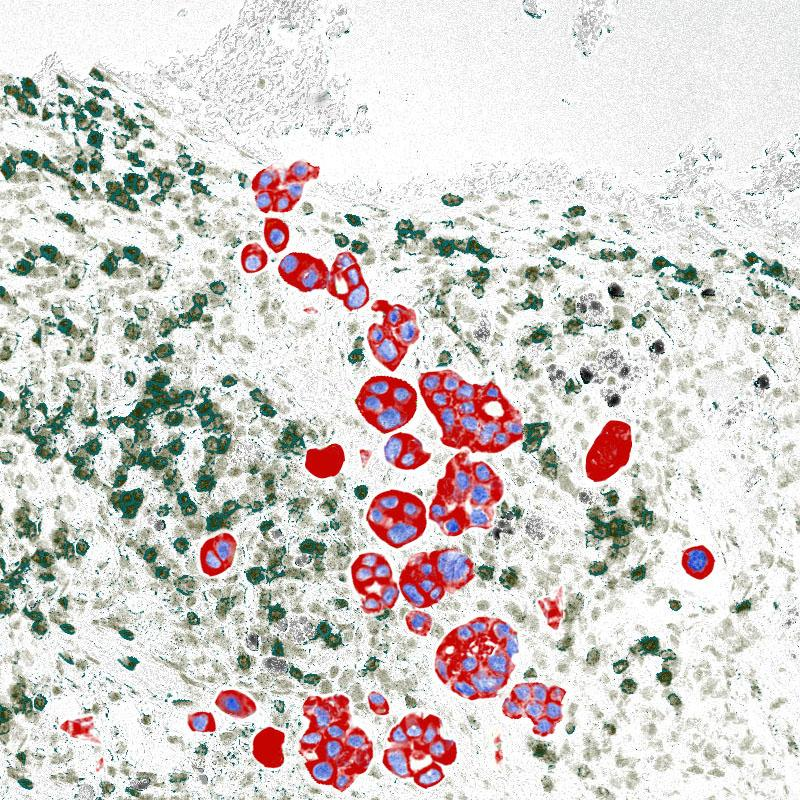
\includegraphics[width=0.8in]{images/possible_image_04.jpg}
}\\
\subfigure{
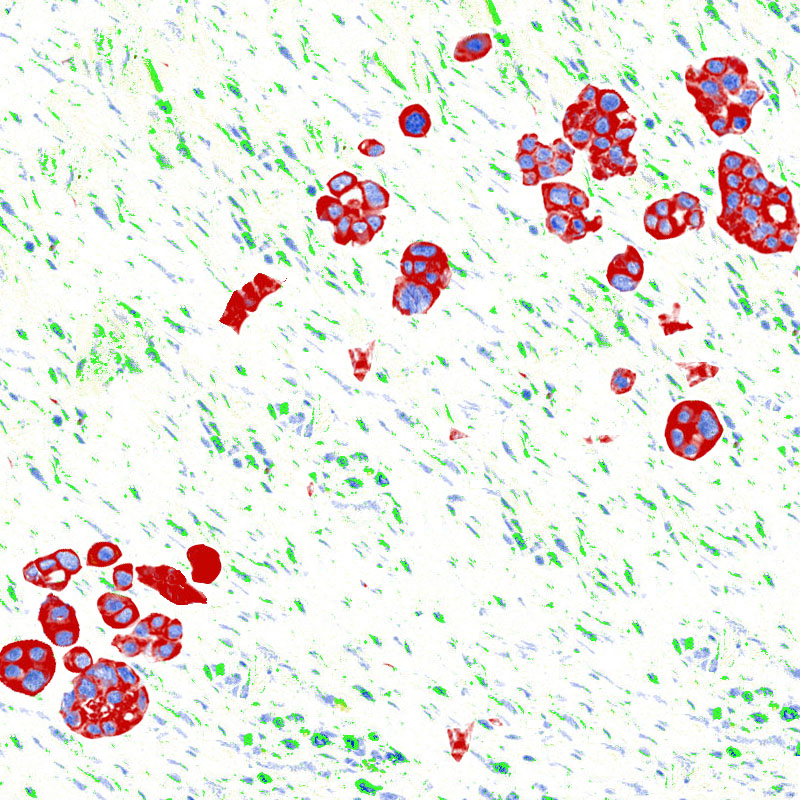
\includegraphics[width=0.8in]{images/possible_image_05.jpg}
}
\subfigure{
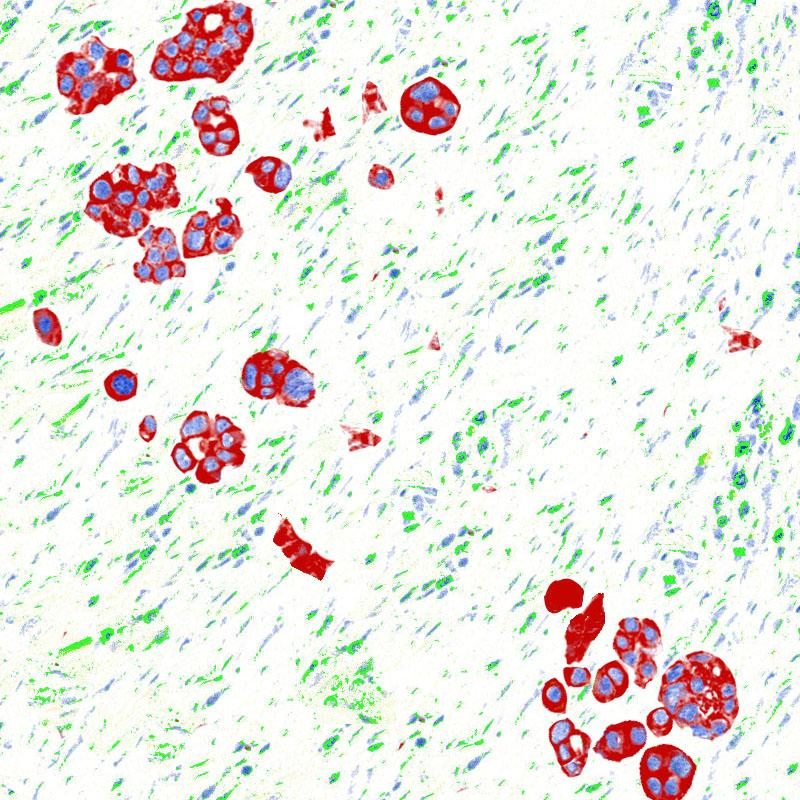
\includegraphics[width=0.8in]{images/possible_image_06.jpg}
}
\subfigure{
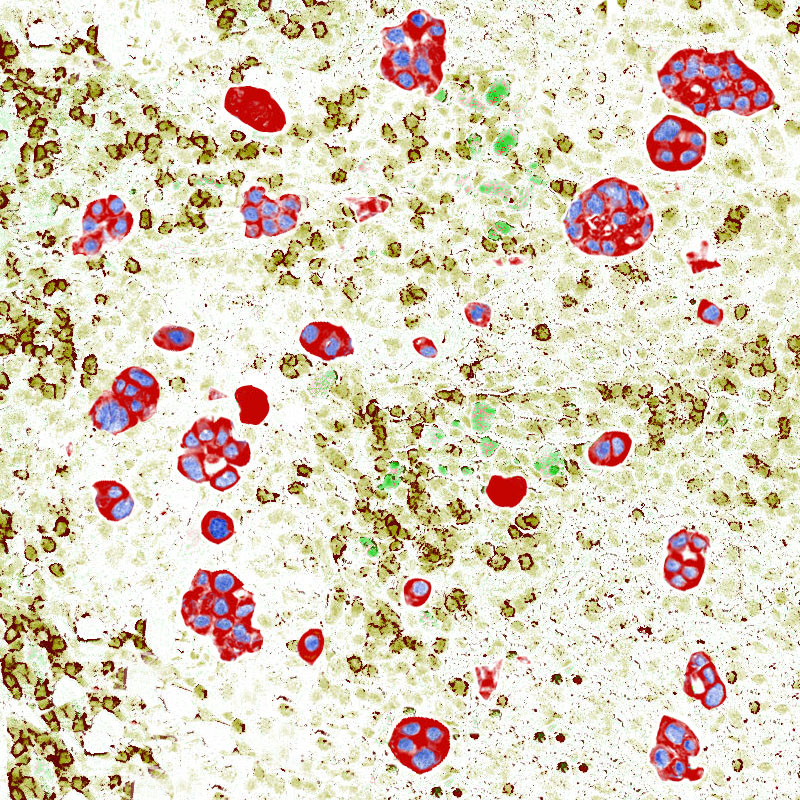
\includegraphics[width=0.8in]{images/possible_image_07.jpg}
}
\subfigure{
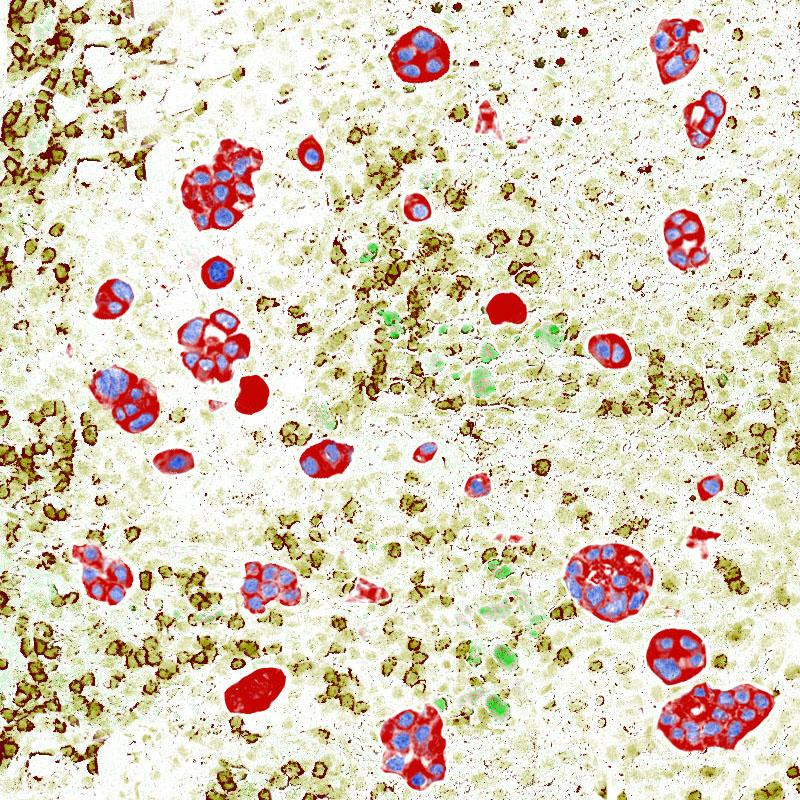
\includegraphics[width=0.8in]{images/possible_image_08.jpg}
}\\
\subfigure{
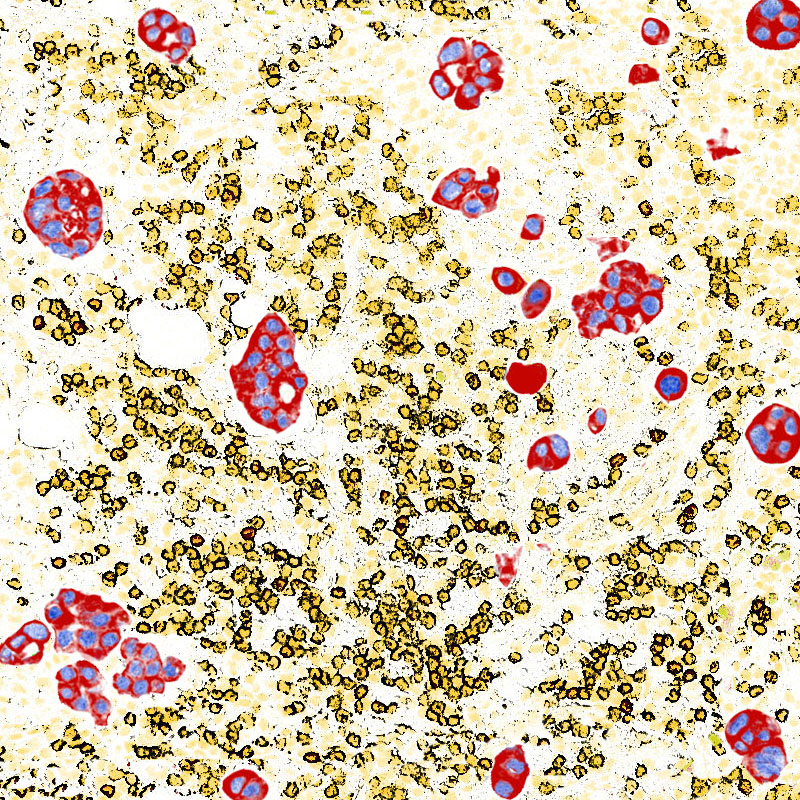
\includegraphics[width=0.8in]{images/possible_image_09.jpg}
}
\subfigure{
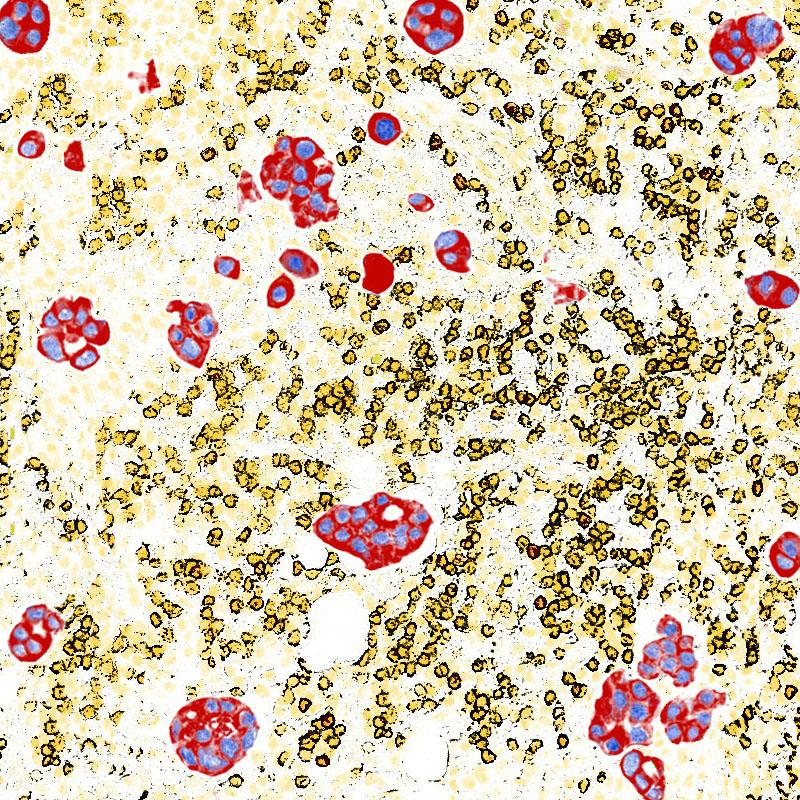
\includegraphics[width=0.8in]{images/possible_image_10.jpg}
}
\end{figure}

\end{frame}
%%%%%%%%%%%%%%%%%%%%%%%%%%%%%%%%%%%%%%%%%%%

%%%%%%%%%%%%%%%%%%%%%%%%%%%%%%%%%%%%%%%%%%%
\begin{frame}\frametitle{The Experimental Flow}

\centeredimage{3.3}{schematic.jpg}

\end{frame}
%%%%%%%%%%%%%%%%%%%%%%%%%%%%%%%%%%%%%%%%%%%

%%%%%%%%%%%%%%%%%%%%%%%%%%%%%%%%%%%%%%%%%%%
\begin{frame}\frametitle{Outcome metrics}

\begin{itemize}
\item Attrition: when did the worker leave? \pause
\item Number of images labeled \pause
\item Quality / Accuracy of labeling:

\beqn
\text{precision} &=& \frac{TP}{TP + FP} \\
\ingreen{\text{recall}} &=& \ingreen{\frac{TP}{TP + FN}} \\
\text{F-measure} &=& 2 \frac{\text{precision} \times \text{recall}}{\text{precision} + \text{recall}} \\
\text{average centrality} &=& \frac{1}{n} \sum_{i=1}^n |\vec{p}_{i_{\text{trained}}} - \vec{p}_{i_{\text{true}}}|
\eeqn

\fbox{fine quality: recall at 2px}
\end{itemize}

\end{frame}
%%%%%%%%%%%%%%%%%%%%%%%%%%%%%%%%%%%%%%%%%%%

%%%%%%%%%%%%%%%%%%%%%%%%%%%%%%%%%%%%%%%%%%%
\begin{frame}\frametitle{Admin Portal: Dashboard}

\centeredimage{4}{dashboard.jpg}

\end{frame}
%%%%%%%%%%%%%%%%%%%%%%%%%%%%%%%%%%%%%%%%%%%

%%%%%%%%%%%%%%%%%%%%%%%%%%%%%%%%%%%%%%%%%%%
\begin{frame}\frametitle{Controlling for time-of-day effects}

\begin{center}
\texttt{
0 * * * * /usr/local/bin/ruby -C \\
../public/web/current/script/runner \\
``HITMaker.create\_hit\_sets(1000)'' -e production}
\end{center}

\vspace{0.5cm}

Create 1000 HITs every hour, on the hour via Linux's \qu{CRON jobs.} Then just wait as the data rolls in. \pause

\centeredimage{1.3}{crank_out_data.jpg}

Just crank out the data...

\end{frame}
%%%%%%%%%%%%%%%%%%%%%%%%%%%%%%%%%%%%%%%%%%%

%%%%%%%%%%%%%%%%%%%%%%%%%%%%%%%%%%%%%%%%%%%
\begin{frame}\frametitle{Admin Portal: Subject Analytics}

\centeredimage{3.3}{training_analytics.jpg}

\end{frame}
%%%%%%%%%%%%%%%%%%%%%%%%%%%%%%%%%%%%%%%%%%%

%%%%%%%%%%%%%%%%%%%%%%%%%%%%%%%%%%%%%%%%%%%
\begin{frame}\frametitle{Admin Portal: Labeling Analytics}

\centeredimage{3.3}{image_analytics.jpg}

\end{frame}
%%%%%%%%%%%%%%%%%%%%%%%%%%%%%%%%%%%%%%%%%%%

%%%%%%%%%%%%%%%%%%%%%%%%%%%%%%%%%%%%%%%%%%%
\begin{frame}\frametitle{Main Results}

$n=2,471$ \pause in 36 days, \inred{68 subjects / day} \\ \pause

Total cost: \$789  \pause (31\cent ~/ subject),  \pause total time labored: 701hr \pause

\centeredimage{4}{bmom_results.jpg}

\centering
Baseline for zero context group: \\
76\% / 37\% / 65\% / \$1.41

\end{frame}
%%%%%%%%%%%%%%%%%%%%%%%%%%%%%%%%%%%%%%%%%%%

%%%%%%%%%%%%%%%%%%%%%%%%%%%%%%%%%%%%%%%%%%%
\begin{frame}\frametitle{25\% of Turkers left feedback }
 \pause 

\scriptsize

\textbf{Meaningful}

\vspace{0.2cm}

\qu{I am hoping you will be offering more HITs like these in the future. It's always nice to have a requester with HITs that do take some thought and mean something to complete} \\

\qu{nice goal i was a cancer patient i respect the efforts of the researchers} \\

\qu{Was this really for research, or was this a social psych experiment?} \\

\qu{I kept thinking of the persons for whom I was confirming the presence of cancer cells, somewhat like I was reading out the death sentence to them. I felt good at completing this task professionally, but there was a profound sense of sadness.}

\vspace{0.2cm} \pause

\textbf{Zero-Context}

\vspace{0.2cm}

\qu{Didn't see the point of doing, only kept doing in hopes of payout increasing} \\

\qu{Tell people what it is accomplishing to make more interesting.} \\

\qu{I'm wondering if this isn't actually a psychological test seeing how low people would go (monetary wise)} \\

\vspace{0.2cm} \pause

\textbf{Shredded}

\vspace{0.2cm}

\qu{That was sort of fun. I have no idea what the point of it was though.} \\

\qu{I felt a little silly since the results weren't going to be used aside from testing.} \\

\qu{Here's a HIT I'd really like to know the purpose of!}

\end{frame}
%%%%%%%%%%%%%%%%%%%%%%%%%%%%%%%%%%%%%%%%%%%

%%%%%%%%%%%%%%%%%%%%%%%%%%%%%%%%%%%%%%%%%%%
\begin{frame}\frametitle{Data Analysis}

\small

Simple linear model, test coefficient of treatment indicators:

\beqn
Y &=& \beta_0 + \beta_T \indic{T} + \beta_1 X_1 + \ldots + \beta_p X_p + \errorrv, \\
\errorrv &\sim& \multnormnot{n}{0}{\sigsq\I_n}
\eeqn

 \pause


For quality, we use quality metrics for each image in a Turker's portfolio. Either use a random intercept model or cluster the standard errors:

\beqn
Y &=& \beta_0 + \gamma_w + \beta_T \indic{T} + \beta_1 X_1 + \ldots + \beta_p X_p + \errorrv, \\
\errorrv &\sim& \multnormnot{n}{0}{\sigsq\I_n} \quad \text{or...} \pause \\
Y &=& \beta_0 + \beta_T \indic{T} + \beta_1 X_1 + \ldots + \beta_p X_p + \errorrv, \\
\errorrv &\sim& \multnormnot{n}{0}{\sigsq\bracks{\begin{array}{cccc} 
D & 0 & \ldots & 0 \\
0 & D & \ldots & 0 \\
 &  & \ddots &  \\
0 & \ldots & 0 & D 
\end{array}}}, \quad D =
\bracks{\begin{array}{cccc} 
1 & \rho & \ldots & \rho \\
\rho & 1 & \ldots & \rho \\
 &  & \ddots &  \\
\rho & \ldots & \rho & 1 \\
\end{array}}
\eeqn

\end{frame}
%%%%%%%%%%%%%%%%%%%%%%%%%%%%%%%%%%%%%%%%%%%

%%%%%%%%%%%%%%%%%%%%%%%%%%%%%%%%%%%%%%%%%%%
\begin{frame}\frametitle{Induced to work $\Leftrightarrow$ Selection Bias}

\small

We do not recommend using induced to work. Turkers have a reputation and \qu{returned HITs} are counted against them. This is most likely the reason there wasn't too much variability. \\ \pause 

\vspace{0.2cm}

However, \textit{leaving} the HIT produces problems. The problem is you cannot observe $y_i$ for the subject who jumped ship. \\ \pause 

\vspace{0.2cm}

Solutions to this missing data problem? \pause  
\begin{itemize}
\item Listwise deletion? Maybe, but it's quite possible opting-out is \textit{non-ignorable}. \pause 
\item Multiple imputation using known covariates? Maybe, unless $\rho(X_j,Y)$'s are large, this is as good as using $\ybar$. \pause 
\item Create dummy variables? Yes, Angrist (2001) recommends using dummies. We used \qu{Labeled more than 5 images?} --- the opt-out's become 0's, and you can run a valid regression. \pause 
\item Conditional-on-positive regression? Yes, as long as you tell your reader. We used \qu{fine quality} \textit{conditional} on being induced-to-work.
\end{itemize}

\end{frame}
%%%%%%%%%%%%%%%%%%%%%%%%%%%%%%%%%%%%%%%%%%%

%%%%%%%%%%%%%%%%%%%%%%%%%%%%%%%%%%%%%%%%%%%
\begin{frame}\frametitle{Group Project}

\centering

Spend 5min with your neighbor coming up with an experiment.

\centeredimage{2}{group_project.jpg}

We'll discuss feasibility of projects.

\end{frame}
%%%%%%%%%%%%%%%%%%%%%%%%%%%%%%%%%%%%%%%%%%%

%%%%%%%%%%%%%%%%%%%%%%%%%%%%%%%%%%%%%%%%%%%
\begin{frame}\frametitle{Internal and Statistical Validity}

Are the causal conclusions in a randomized MTurk experiment warranted? \\

\vspace{0.2cm}

If anything, it's more internally valid than a lab experiment (as long as differential attrition is taken care of).  \pause There's no experimenter bias,  \pause perfect blinding --- disinterested randomization, \pause  SUTVA --- better than the lab. \\ \pause 

\vspace{0.2cm}

Statistical conclusion validity: we have much higher power versus lab experiments ($n \approx 2,500$ in our example).

\end{frame}
%%%%%%%%%%%%%%%%%%%%%%%%%%%%%%%%%%%%%%%%%%%

%%%%%%%%%%%%%%%%%%%%%%%%%%%%%%%%%%%%%%%%%%%
\begin{frame}\frametitle{External Validity / Generalizability}

\small

Berinsky et al (2012) demonstrated that at least in the US, experimental results can be \textit{generalized} to the American population at large unless you suspect heterogeneous effects:

\beqn
Y &=& \beta_0 + \beta_T \indic{T} + \beta_1 X_1 + \ldots + \beta_p X_p + \underbrace{h(\indic{T}, X_1, \ldots, X_p)}_{\text{large?}} +  \errorrv, \\
\errorrv &\sim& \multnormnot{n}{0}{\sigsq\I_n}
\eeqn
 \pause 
They gave some of the covariates that could be problematic: age, political ideology, political knowledge, etc. However, there is no guarantee there aren't \textit{other} covariates that they didn't explore. It is better than convenience samples. \pause 

\vspace{0.2cm}

External Validity is \textit{never} airtight! But it looks promising for MTurk vis-a-vis most published lab studies. \pause 

\vspace{0.2cm}

Ecological validity? Maybe not... but that always depends!

\end{frame}
%%%%%%%%%%%%%%%%%%%%%%%%%%%%%%%%%%%%%%%%%%%

%%%%%%%%%%%%%%%%%%%%%%%%%%%%%%%%%%%%%%%%%%%
\begin{frame}\frametitle{Why do we care? Natural field Experiments}

\centeredimage{4}{lab_vs_field.jpg}

\begin{quotation}
\inred{\textsc{external validity problems}}``...lab 
experiments in isolation are necessarily limited in relevance for
predicting field behavior, unless one wants
to insist a priori that those aspects of economic
behavior under study are perfectly
general...'' -Harrison and List (2004)
\end{quotation}

\end{frame}
%%%%%%%%%%%%%%%%%%%%%%%%%%%%%%%%%%%%%%%%%%%

%%%%%%%%%%%%%%%%%%%%%%%%%%%%%%%%%%%%%%%%%%%
\begin{frame}\frametitle{Natural field Experiments on MTurk}

Why are natural field experiments on MTurk \textit{better} than most natural field experiments? Evaluated by the Levitt and List (2007, 2009) rubric: \pause 

\begin{itemize}
\scriptsize
\item \ingreen{scrutiny and anonymity:}  \pause No \qu{Hawthorne effects:} Turkers don't know they're being watched.  \pause No \qu{Clever Hans effects:} Turkers cannot respond to the researcher's subtle cues. In fact, no interaction with the experimenter since they don't know they're in an experiment!
\item \ingreen{artificial restrictions:}  \pause the Turkers are allowed to perform the task however they please (within a time limit).
\item \ingreen{need for cooperation with third parties:}  \pause none!
\item \ingreen{difficulty of replication:}  \pause \texttt{git clone}, load up the account with money --- perfect, push-button replication!
\end{itemize}

Possible issues

\begin{itemize}
\scriptsize
\item \inred{Stakes:}  \pause You can argue the wages on MTurk are too low to generalize. \pause
\item \inred{Selection:}  \pause Are Turkers different from the rest of the population. Berinsky et al say \qu{no} but there is room to say \qu{yes.}
\end{itemize}

\end{frame}
%%%%%%%%%%%%%%%%%%%%%%%%%%%%%%%%%%%%%%%%%%%

%%%%%%%%%%%%%%%%%%%%%%%%%%%%%%%%%%%%%%%%%%%
\begin{frame}\frametitle{Ethical Issues}

Research using human subjects has to pass an \textit{institutional review board} (IRB) review process. Simple surveying and labeling tasks on adults are \textit{exempt} from review under \qu{category 2.}  \pause However, you may have noticed we used a fake name and \textit{never} told the Turkers they were in an experiment in order to create a \textit{natural field experiment} which is a form of...

\centeredimage{2}{deception.jpg} \pause 

Thus, this study had to pass a \textit{full board} IRB meeting and we needed to provide justification. \pause  They also asked us to send a debrief message to all subjects post-experiment.

\end{frame}
%%%%%%%%%%%%%%%%%%%%%%%%%%%%%%%%%%%%%%%%%%%

%%%%%%%%%%%%%%%%%%%%%%%%%%%%%%%%%%%%%%%%%%%
\begin{frame}\frametitle{Some literature on MTurk experimentation}

\scriptsize 
\vspace{0.2cm}

\begin{itemize}
\item Multi-player MTurk experiment tests altruism and cooperation under various \qu{local public goods} games. (Suri and Watts, 2011) \pause
\item Replicating classical Tversky-Kahneman-type psychological experiments finds agreement with effect sizes. (Horton et al., 2011)  \pause
\item Does \qu{honesty priming} make Turkers more willing to admit to self-destructive alcoholic binges? (Pashler et al., 2013)  \pause
\item Relying on \qu{intuition} over \qu{reasoning} causes about 30\% more risk tolerance. (Butler et al., 2013) \pause
\end{itemize}
\vspace{0.2cm}

\textbf{Further reading on MTurk as a platform}

\begin{itemize}
\scriptsize
\item \qu{Conducting behavioral research on Amazon's Mechanical Turk} (Mason and Suri, 2012)
\item \qu{The promise of Mechanical Turk: how online labor markets can help theorists run behavioral experiments} (Rand, 2012)
\item \qu{Evaluating Amazon's Mechanical Turk as a tool for experimental behavioral research} (Crump et al, 2013)
%\item \qu{Separate but equal? A comparison of participants and data gathered via Amazon’s MTurk, social media, and face-to-face behavioral testing} (Casler et al, 2013)
\end{itemize}

\end{frame}
%%%%%%%%%%%%%%%%%%%%%%%%%%%%%%%%%%%%%%%%%%%

%%%%%%%%%%%%%%%%%%%%%%%%%%%%%%%%%%%%%%%%%%%
\begin{frame}\frametitle{Checkpoint}

We've covered:

\begin{itemize}
\item a case study examining an MTurk experiment in detail \pause
\item a group exercise designing an experiment \pause
\item issues to look out for during analysis \pause
\item internal and external validity when drawing conclusions from the data \pause
\item MTurk as a platform for high-power \textit{natural field experiments} \pause
\end{itemize}

\begin{block}{Goal D Complete}
\small
\begin{enumerate}
\item[D] For crowdsourced randomized experiments:
\begin{itemize}
\item Evaluate if the experiment is suitable for crowdsourcing
\item Design the experiment
\item Analyze the resulting data
\end{itemize}
\end{enumerate}
\end{block}

\end{frame}
%%%%%%%%%%%%%%%%%%%%%%%%%%%%%%%%%%%%%%%%%%%

\section{Further Devs}

%%%%%%%%%%%%%%%%%%%%%%%%%%%%%%%%%%%%%%%%%%%
\begin{frame}\frametitle{Further Developments: Some extensions and plugins in the literature}

 \pause

\small

\begin{itemize}
\item \qu{UserActionTracer}  (Stieger and Reips, 2010) collects \textit{paradata} (information about mouse clicks, mouse movements, keystrokes) that we believe can be used in MTurk labeling tasks to inform quality of the label, and in experiments admitting better covariates and increasing efficiency of estimates.   \pause
\item  \qu{Soylent} (Bernstein et al., 2010)  is a word processing interface that embeds crowdsourcing labor. It helps users write by being able to have Turkers complete annoying find-fix-verify tasks such as text shortening, spelling and grammar checking, and formating citations and finding figures.  \pause
\item Little et al (2010) studied tasks broken up iteratively or in parallel for many different types of microtasks. They found that iterative work on a task increases the average accuracy, but many Turkers in parallel increase the maximum accuracy.
\end{itemize}

\end{frame}
%%%%%%%%%%%%%%%%%%%%%%%%%%%%%%%%%%%%%%%%%%%

%%%%%%%%%%%%%%%%%%%%%%%%%%%%%%%%%%%%%%%%%%%
\begin{frame}\frametitle{Further Developments: Use MTurk to study Statistical Questions}
 \pause

We talked a bit about heterogeneous effects where the conclusions of a study may not be applicable to the population of interest. Many experiments in the real world are run by recruiting subjects who \textit{want} to be in the study.  \pause

\vspace{0.2cm}

Does \textit{wanting} to be in the study affect the \textit{average treatment effect}? Is there selection bias \textit{into} the randomized trial itself? This can be tested.

\end{frame}
%%%%%%%%%%%%%%%%%%%%%%%%%%%%%%%%%%%%%%%%%%%

%%%%%%%%%%%%%%%%%%%%%%%%%%%%%%%%%%%%%%%%%%%
\begin{frame}\frametitle{An experiment to test a statistical phenomenon}

\centeredimage{3}{sel_bias_experimental_setup.jpg}

\centering
Design flowchart for proposed experiment

\end{frame}
%%%%%%%%%%%%%%%%%%%%%%%%%%%%%%%%%%%%%%%%%%%


%%%%%%%%%%%%%%%%%%%%%%%%%%%%%%%%%%%%%%%%%%%
\begin{frame}\frametitle{Power calculation}

\beqn
F^* &:=& F(95\%,1, 4(r-1)), \quad W \sim F\parens{1, 4(r-1), \frac{4r\beta_{ST}^2}{\sigsq}}, \\
\text{POW} &:=& \prob{W > F^*}, \quad\quad \sigsq \approx 12.8 ~~\text{(from pilot data)}
\eeqn

\tiny
Let $r$ be the number of duplicates, $N$ is total sample size, $\sigsq$ is the variance of the homoskedastic error term, and $\beta_{ST}$ is the true interaction effect between selecting the study and treatment. \pause


\begin{table}[htp]
\begin{center}
\small
\begin{tabular}{c|c|cccccccc}
 & & \multicolumn{8}{c}{$\beta_{ST}$ (\$)} \\
$N_{\text{study}}$ & $r$  & 0.01 & 0.05 & 0.1 & 0.15 & 0.2 & 0.25 & 0.5 & 0.75 \\ 
  \hline
400 & 100 & 0.05 & 0.06 & 0.09 & 0.14 & 0.22 & 0.31 & 0.84 & 0.99 \\ 
800 &  200 & 0.05 & 0.07 & 0.13 & 0.24 & 0.39 & 0.55 & 0.99 & 1.00 \\ 
1200 &  300 & 0.05 & 0.08 & 0.18 & 0.34 & 0.53 & 0.73 & 1.00 & 1.00 \\ 
1600 &   400 & 0.05 & 0.09 & 0.22 & 0.43 & 0.66 & 0.84 & 1.00 & 1.00 \\ 
2000 &  500 & 0.05 & 0.10 & 0.26 & 0.51 & 0.75 & 0.91 & 1.00 & 1.00 \\ 
2400 &  600 & 0.05 & 0.11 & 0.30 & 0.58 & 0.83 & 0.95 & 1.00 & 1.00 \\ 
2800 &  700 & 0.05 & 0.12 & 0.35 & 0.65 & 0.88 & 0.97 & 1.00 & 1.00 \\
\end{tabular}
\end{center}
\end{table}
\normalsize

\colorbox{yellow}{Began thinking: how can I reduce $\sigsq$?}

\end{frame}
%%%%%%%%%%%%%%%%%%%%%%%%%%%%%%%%%%%%%%%%%%%

%%%%%%%%%%%%%%%%%%%%%%%%%%%%%%%%%%%%%%%%%%%
\begin{frame}\frametitle{Current Research: Matching to Reduce Variance}

\begin{quotation}
``Perhaps the best way of reducing the error due to differences between person is to match \textit{before} random assignments to treatments.''
\end{quotation}

\begin{thebibliography}{1}
\bibitem{breiman2001}
\tiny
Cook, Thomas D., and Donald T. Campbell. "Quasi-experimentation: Design and analysis for field setting." MA: Houghton Mifflin (1979).
\end{thebibliography} \pause

\beqn
\Y &=& \beta_T \indic{T} + \X\bbeta + \berrorrv, \quad \var{\berrorrv} = \sigsq_e\I_n \\
\expe{\Ybar_T - \Ybar_C} &=& \beta_T \eqncomment{expectorating over $\indic{T}$} \\
\var{\Ybar_T - \Ybar_C} &=& \bbeta^\top \var{\Xbar_T - \Xbar_C} \bbeta + \underbrace{\var{\bar{\berrorrv}_T - \bar{\berrorrv}_C}}_{\approx 4\sigsq_e/n}
\eeqn

\vspace{-0.5cm}
\begin{thebibliography}{1}
\bibitem{breiman2001}
\tiny
Morgan, K. L., \& Rubin, D. (2012). Rerandomization to improve covariate balance in experiments. The Annals of Statistics, 40(2), 1263---1282
\end{thebibliography} \pause

If the sample averages of the $x$'s in each group are balanced, the variance drops.

\end{frame}
%%%%%%%%%%%%%%%%%%%%%%%%%%%%%%%%%%%%%%%%%%%

%%%%%%%%%%%%%%%%%%%%%%%%%%%%%%%%%%%%%%%%%%%
\begin{frame}\frametitle{Matching to Reduce Variance}

Most real world data is \qu{nonlinear.} This is our focus. \pause

\beqn
\Y &=& \beta_T \indic{T} + \z + \berrorrv, \quad z_i := f(x_{1i}, \ldots, x_{pi})\\
\expe{\Ybar_T - \Ybar_C} &=& \beta_T \eqncomment{expectorating over $\indic{T}$} \\
\var{\Ybar_T - \Ybar_C} &=& \var{\Zbar_T - \Zbar_C} + \underbrace{\var{\bar{\berrorrv}_T - \bar{\berrorrv}_C}}_{\approx 4\sigsq_e/n}
\eeqn

Same mechanism in a non-linear model. \pause


\begin{itemize}
\item if for all subjects $f(\x_{T,i}) \approx f(\x_{C,i})$ (balance between treatment and control), we achieve a more efficient estimator on average over many experiments \pause
\item if $n_T \approx n_C$ we also achieve a more efficient estimator
\end{itemize}

\end{frame}

\begin{frame}
	\frametitle{Student's Identical-Twins Idea (1931)}

\begin{figure}[htp]
\centering
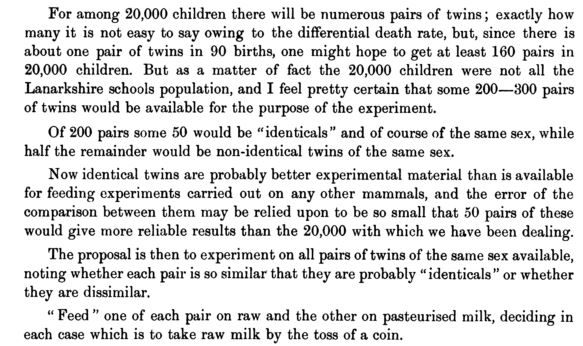
\includegraphics[width=3.4in]{images/student.jpg}
\end{figure}

\end{frame}
%%%%%%%%%%%%%%%%%%%%%%%%%%%%%%%%%%%%%%%%%%%

%%%%%%%%%%%%%%%%%%%%%%%%%%%%%%%%%%%%%%%%%%%
\begin{frame}\frametitle{Back to MTurk: Sequential Experiment}

Subjects enter sequentially and must immediately be assigned treatment or control. \pause What if we match ``on-the-fly?'' \pause

\vspace{-0.25cm}
\begin{table}[htp]
\begin{center}
\small
\begin{tabular}{cccccccc}
$t$ &Subject & Age & Gender & Likes donuts? & Smokes? & Smart? & $\indic{T}$ \\ \hline \vspace{0.25cm} \pause
1 & 
\includegraphics[width=0.4in]{images/homer.jpg} & 40 & M & Y & N & N & \pause T \pause\\
2 & 
\includegraphics[width=0.4in]{images/selma.jpg} & 46 & F & N & Y & Y & \pause C \pause\\
3 & 
\includegraphics[width=0.4in]{images/apu.jpg} & 46 & M & Y & N & Y & \pause C \pause\\
4 & 
\includegraphics[width=0.4in]{images/patty.jpg} & 46 & F & N & Y & Y & \pause T \pause\\
5 & 
\includegraphics[width=0.4in]{images/wiggum.jpg} & 48 & M & Y & Y & N &  \pause C \\
\end{tabular}
\end{center}
\end{table}

\end{frame}
%%%%%%%%%%%%%%%%%%%%%%%%%%%%%%%%%%%%%%%%%%%

%%%%%%%%%%%%%%%%%%%%%%%%%%%%%%%%%%%%%%%%%%%
\begin{frame}\frametitle{The ``Reservoir'' and the ``Matches''}

\only<1>{
$t=1$

\begin{figure}[htp]
\centering

\includegraphics[width=4in]{images/sim_t_1.jpg}
\end{figure}
}
\only<2>{
$t=2$

\begin{figure}[htp]
\centering
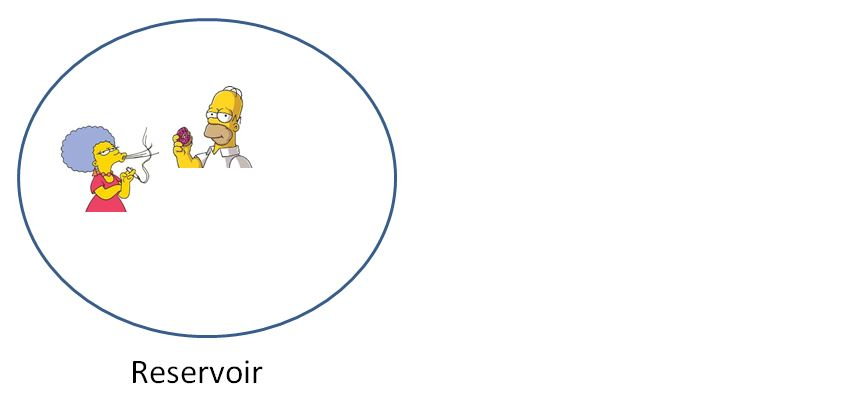
\includegraphics[width=4in]{images/sim_t_2.jpg}
\end{figure}
}
\only<3>{
$t=3$

\begin{figure}[htp]
\centering
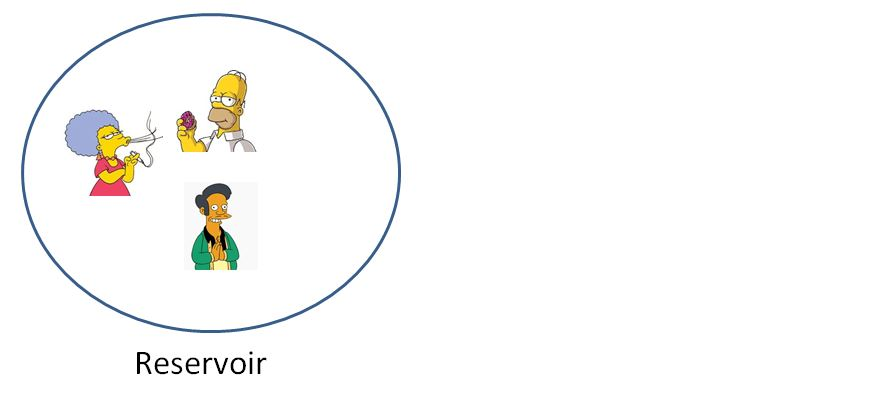
\includegraphics[width=4in]{images/sim_t_3.jpg}
\end{figure}
}
\only<4>{
$t=4$

\begin{figure}[htp]
\centering
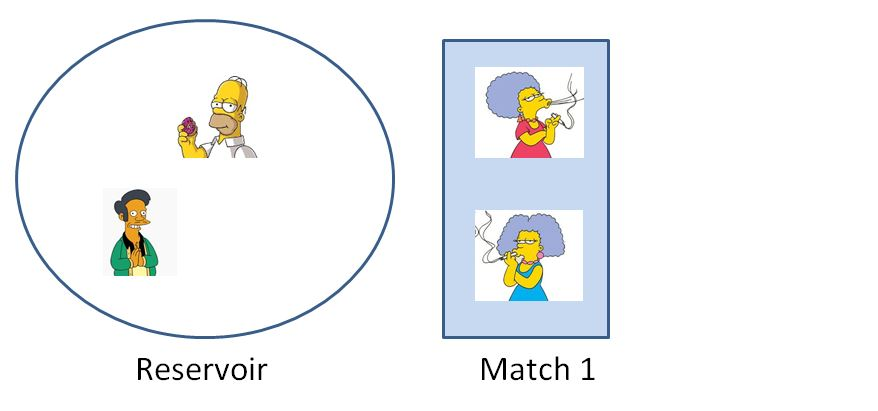
\includegraphics[width=4in]{images/sim_t_4.jpg}
\end{figure}
}
\only<5>{
$t=5$

\begin{figure}[htp]
\centering
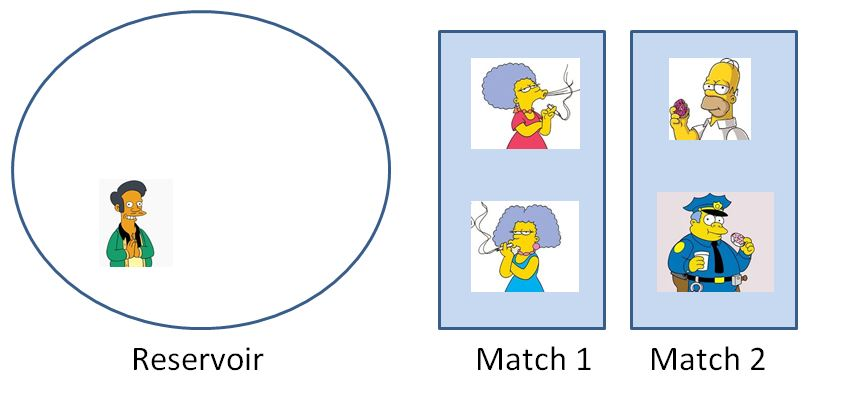
\includegraphics[width=4in]{images/sim_t_5.jpg}
\end{figure}
}

\pause

Ending stats $n_R = 1, ~m=2$. 
\end{frame}
%%%%%%%%%%%%%%%%%%%%%%%%%%%%%%%%%%%%%%%%%%%


%%%%%%%%%%%%%%%%%%%%%%%%%%%%%%%%%%%%%%%%%%%
\begin{frame}\frametitle{How to match?}

Matching on Mahalanobis distance. Assume covariates are normal enough to use the scaled $F$ distribution.

\begin{thebibliography}{1}
\bibitem{breiman2001}
\tiny
Greevy, R., Lu, B., Silber, J. H., \& Rosenbaum, P. Optimal multivariate matching before randomization. Biostatistics (2004), 5(2), 263---75
\end{thebibliography} \pause

\newcommand{\xnew}{\x_{\text{new}}}
\newcommand{\xold}{\x_{\text{old}}}
\newcommand{\Xnew}{\X_{\text{new}}}
\newcommand{\Xold}{\X_{\text{old}}}

\beqn\label{eq:mahalanobis}
D^2_M := \oneover{2} (\Xnew - \Xold)^\top \bv{S}^{-1} (\Xnew - \Xold), \quad  \frac{n-p}{p(n-1)}D^2_M  \sim F_{p,n-p}
\eeqn

Choose a $\pval$ hyperparameter, $\lambda \in (0,1)$, to represent the cutoff probability to match: the higher $\lambda$ is, the easier to match.


\end{frame}
%%%%%%%%%%%%%%%%%%%%%%%%%%%%%%%%%%%%%%%%%%%

%%%%%%%%%%%%%%%%%%%%%%%%%%%%%%%%%%%%%%%%%%%
\begin{frame}\frametitle{The Sequential Match Classic Estimator}

Consider $H_0: \beta_T = \beta_0$ versus $H_a: \beta_T \neq \beta_0$. \\ \pause \vspace{0.25cm}
Since $\SsqDbar \convp \sigsqDbar$ and $\SsqR \convp \sigsqR$, we now have a $Z$-like testing estimator: \pause

\beqn\label{eq:clt_true_var}
\frac{B_T - \beta_0}{\se{B_T}} \approx \frac{\dfrac{\SsqR \Dbar + \SsqDbar \parens{\YbarRTMinusYbarRC}}{\SsqR + \SsqDbar} - \beta_0}{\sqrt{\dfrac{\SsqR\SsqDbar}{\SsqR + \SsqDbar}}}  ~\convd~ \stdnormnot
\eeqn
\pause
Note that in the case where there are no matched pairs, we default to the classic estimator and in the case where there are less than two treatments or controls in the reservoir, we use only the matched pairs component.

\end{frame}
%%%%%%%%%%%%%%%%%%%%%%%%%%%%%%%%%%%%%%%%%%%

%%%%%%%%%%%%%%%%%%%%%%%%%%%%%%%%%%%%%%%%%%%
\begin{frame}\frametitle{Relative Power}
\small 
Simulate on a non-linear model:

\beqn
&& \beta_T\indic{T,i} + x_{1,i} + x_{2,i} + x_{1,i}^2 + x_{2,i}^2 +x_{1,i} x_{2,i} + \errorrv_i \\
&& X_{1,i} \iid \stdnormnot, \quad X_{2,i} \iid \stdnormnot, \quad \errorrv_i \iid \normnot{0}{\sigsq_e} \\
&& \beta_T = 1, \quad \sigsq_e = 3, \quad N_{\text{sim}} = 1000
\eeqn

\centeredimage{1.6}{model_I_classic.pdf}

\centering
(~\inred{$n=50$}, \ingreen{$n=100$}, \inblue{$n=200$})

\end{frame}
%%%%%%%%%%%%%%%%%%%%%%%%%%%%%%%%%%%%%%%%%%%

%%%%%%%%%%%%%%%%%%%%%%%%%%%%%%%%%%%%%%%%%%%
\begin{frame}\frametitle{Results on a Clinical Trial}

On 200 simulations and using all covariates... \pause

\begin{table}[htp]
\centering
\begin{tabular}{r|ccc}
purported  & actual $n$  & average & approximate sample  \\
 $n$ & (average) & efficiency & size reduction \\ \hline
100 & 75.2 & 1.10 & 9.2\% \\
150 & 111.3 & 1.05 & 4.9\% \\
224 (all) & 165.5 & 1.07 & 6.7\%
\end{tabular}
\end{table}
\pause
Snooping and using the top 4 covariates... \pause

\begin{table}[htp]
\centering
\begin{tabular}{r|ccc}
purported  & actual $n$  & average & approximate sample  \\
 $n$ & (average) & efficiency & size reduction \\ \hline
100 & 72.9 & 1.23 & 18.8\% \\
150 & 108.6 & 1.15 & 13.2\% \\
224 (all) & 160.3 & 1.13 & 11.3\%
\end{tabular}
\end{table}

\end{frame}
%%%%%%%%%%%%%%%%%%%%%%%%%%%%%%%%%%%%%%%%%%%

%%%%%%%%%%%%%%%%%%%%%%%%%%%%%%%%%%%%%%%%%%%
\begin{frame}\frametitle{How do we pretend to use our sequential matching procedure?}
% is this needed or is it just a technical detail?

\centeredimage{4.5}{real_data_sims.jpg}

Note that sometimes $\bv{S}_t^{-1}$ cannot be inverted, so we use the Moore-Penrose generalized inverse.

\end{frame}
%%%%%%%%%%%%%%%%%%%%%%%%%%%%%%%%%%%%%%%%%%%


%%%%%%%%%%%%%%%%%%%%%%%%%%%%%%%%%%%%%%%%%%%
\begin{frame}\frametitle{Remember the MTurk data block structure}

\small

Machine Learning usually expects: \pause

\beqn
Y_i = f(x_{1i}, \ldots, x_{pi}) + \errorrv_i, \quad \errorrv_1, \ldots, \errorrv_n \iid e(0, \sigsq) \pause
\eeqn

What does data from MTurk \textit{really} look like? \pause

\begin{minipage}{0.60\linewidth}

\centeredimage{2.5}{crowdsourcing_data_format.jpg}

\pause
\end{minipage}
\begin{minipage}{0.38\linewidth}
Thus, $n_{\text{eff}} \in \bracks{12, 31}$, \pause an inconvenient reality that off-the-shelf ML algorithms do not consider:\\ \pause

\footnotesize
\beqn
\berrorrv \sim e\parens{\zerovec,~ \sigsq\threebythreemat{\D_1}{}{}{}{\ddots}{}{}{}{\D_{12}}}
\eeqn

\end{minipage}

\end{frame}
%%%%%%%%%%%%%%%%%%%%%%%%%%%%%%%%%%%%%%%%%%%

%%%%%%%%%%%%%%%%%%%%%%%%%%%%%%%%%%%%%%%%%%%
\begin{frame}\frametitle{A new machine learning method to use block structure}

\scriptsize
\qu{Bayesian Additive Regression Trees} (Chipman et al, 2010) is a machine learning method that builds a sum-of-trees model using a normal likelihood for node data and various priors to control regularization:


\beqn
\Y = \underbrace{\treet{1}^\leaf (\X) + \treet{2}^\leaf (\X) + \ldots + \treet{m}^\leaf (\X)}_f + \berrorrv, \quad\quad \berrorrv \sim \multnormnot{n}{\zerovec}{\sigsq\I_n}
\eeqn \pause

and it can be extended to handle

\beqn
\Y = \treet{1}^\leaf (\X) + \treet{2}^\leaf (\X) + \ldots + \treet{m}^\leaf (\X) + \berrorrv, \quad\quad \berrorrv \sim \multnormnot{n}{\zerovec}{\sigsq\threebythreemat{\D_1}{}{}{}{\ddots}{}{}{}{\D_{k}}}
\eeqn \pause

\vspace{-0.2cm}

where the block structure could be compound symmetric: \pause

\beqn
\D = \bracks{\begin{array}{cccc} 
1 & \rho & \cdots & \rho \\
\rho & 1 & \cdots & \rho \\
\vdots & \vdots & \ddots & \vdots \\
\rho & \rho & \cdots & 1 \\
\end{array}}, \quad\quad \rho \sim \prob{\cdot}
\eeqn
\pause
$\rho$ can be estimated for entire data set or inside of each Turker's work portfolio. \\

\end{frame}
%%%%%%%%%%%%%%%%%%%%%%%%%%%%%%%%%%%%%%%%%%%

%%%%%%%%%%%%%%%%%%%%%%%%%%%%%%%%%%%%%%%%%%%
\begin{frame}\frametitle{What we covered}

\begin{itemize}
\item Crowdsourcing and microlabor - a booming field
\item Using MTurk for surveying, collecting labeled data, and experimenting
\item Some issues and research opportunities in collecting and using Mturk-generated data
\end{itemize}

We enjoyed having you all in our tutorial! Questions?

\vspace{1cm}

\scriptsize
\large{\textbf{Acknowledgements}}
\vspace{0.2cm}

\scriptsize
We would like to thank Larry Brown, Dana Chandler, Dean Foster, John Horton, Panos Ipeirotis, Abba Krieger, Mary Putt, Abraham Wyner. Adam acknowledges the NSF for his graduate research fellowship that made this research possible.


\end{frame}
%%%%%%%%%%%%%%%%%%%%%%%%%%%%%%%%%%%%%%%%%%%

\end{document}
